% ============================================================
%  RAPPORT DE FIN D'ANNEE — RISKSIGHT
%  Plateforme SaaS de Scoring du Risque Credit
%  4eme Annee Ingenierie Data Analytics
%  Rania Bikikre & Imane Nadif — 4IAD-G2 — 2025-2026
%
%  COMPILATION : pdfLaTeX (deux passes suffisent)
%  Tout est dans ce seul fichier — aucun .bib externe
% ============================================================

\documentclass[12pt, a4paper]{report}

% ── Encodage & Langue ──────────────────────────────────────
\usepackage[utf8]{inputenc}
\usepackage[T1]{fontenc}
\usepackage[french]{babel}
\usepackage{csquotes}

\usepackage{amssymb}

% ── Mise en page ───────────────────────────────────────────
\usepackage[top=2.5cm, bottom=2.5cm, left=3cm, right=2.5cm]{geometry}
\usepackage{setspace}
\onehalfspacing
\setlength{\headheight}{14pt}

% ── Couleurs ───────────────────────────────────────────────
\usepackage[dvipsnames]{xcolor}
\definecolor{primary}{RGB}{0,82,147}
\definecolor{secondary}{RGB}{255,140,0}
\definecolor{lightgray}{RGB}{245,245,245}
\definecolor{darkgray}{RGB}{80,80,80}
\definecolor{successcolor}{RGB}{34,139,34}
\definecolor{dangercolor}{RGB}{178,34,34}

% ── Graphiques & TikZ ──────────────────────────────────────
\usepackage{graphicx}
\usepackage{float}
\usepackage{tikz}
\usetikzlibrary{shapes.geometric,arrows.meta,positioning,shadows,fit}
\usepackage{pgfplots}
\pgfplotsset{compat=1.18}
\usepackage{pgfgantt} 

% ── Tableaux ───────────────────────────────────────────────
\usepackage{booktabs}
\usepackage{tabularx}
\usepackage{multirow}
\usepackage{array}
\usepackage{colortbl}
\usepackage{longtable}

% ── Listes & Boites ────────────────────────────────────────
\usepackage{enumitem}
\usepackage[most]{tcolorbox}

% ── Code source ────────────────────────────────────────────
\usepackage{listings}
\lstset{
  basicstyle=\ttfamily\small,
  backgroundcolor=\color{lightgray},
  frame=single,
  framerule=0.5pt,
  rulecolor=\color{primary},
  breaklines=true,
  numbers=left,
  numberstyle=\tiny\color{darkgray},
  keywordstyle=\color{primary}\bfseries,
  commentstyle=\color{darkgray}\itshape,
  stringstyle=\color{secondary},
  showstringspaces=false,
  tabsize=2,
  captionpos=b,
  literate=
    {é}{{\'e}}1 {è}{{\`e}}1 {ê}{{\^e}}1 {ë}{{\"e}}1
    {à}{{\`a}}1 {â}{{\^a}}1 {ù}{{\`u}}1 {û}{{\^u}}1
    {î}{{\^i}}1 {ô}{{\^o}}1 {ç}{{\c c}}1
    {É}{{\'E}}1 {È}{{\`E}}1 {Ê}{{\^E}}1
    {À}{{\`A}}1 {Ç}{{\c C}}1
}
\lstdefinelanguage{SQL}{
  keywords={SELECT,FROM,WHERE,JOIN,ON,GROUP,BY,ORDER,HAVING,
            CREATE,TABLE,INSERT,INTO,VALUES,UPDATE,SET,DELETE,
            INDEX,PRIMARY,KEY,FOREIGN,REFERENCES,SCHEMA,USE,
            UNION,ALL,AS,NOT,NULL,IDENTITY,INT,SMALLINT,
            NVARCHAR,FLOAT,DATE,DATETIME,GO,RESEED,DBCC,
            CHECKIDENT,DISTINCT,COUNT,SUM,AVG,MAX,MIN,
            INNER,LEFT,RIGHT,FULL,OUTER,EXISTS,IN},
  sensitive=false,
  morecomment=[l]{--},
  morestring=[b]'
}

% ── En-tetes & Pieds de page ───────────────────────────────
\usepackage{fancyhdr}
\pagestyle{fancy}
\fancyhf{}
\fancyhead[L]{\small\textcolor{primary}{\textsc{RiskSight --- Rapport de Fin d'Ann\'ee}}}
\fancyhead[R]{\small\textcolor{darkgray}{2025--2026}}
\fancyfoot[C]{\thepage}
\fancyfoot[L]{\small\textcolor{darkgray}{Bikikre \& Nadif --- 4IAD-G2}}
\renewcommand{\headrulewidth}{0.4pt}
\renewcommand{\footrulewidth}{0.3pt}

% ── Titres de chapitres ────────────────────────────────────
\usepackage{titlesec}
\titleformat{\chapter}[display]
  {\normalfont\Large\bfseries\color{primary}}
  {\chaptertitlename\ \thechapter}{10pt}{\Huge}
\titleformat{\section}
  {\normalfont\large\bfseries\color{primary}}{\thesection}{1em}{}
\titleformat{\subsection}
  {\normalfont\normalsize\bfseries\color{darkgray}}{\thesubsection}{1em}{}
\titleformat{\subsubsection}
  {\normalfont\normalsize\itshape\color{darkgray}}{\thesubsubsection}{1em}{}

% ── Liens hypertexte ───────────────────────────────────────
\usepackage[hidelinks,colorlinks=true,
            linkcolor=primary,urlcolor=secondary]{hyperref}
\usepackage{url}

% ── Mathematiques ──────────────────────────────────────────
\usepackage{amsmath}

% ── Caption ────────────────────────────────────────────────
\usepackage{caption}

% ── Boites personnalisees (sans fontawesome) ───────────────
\tcbset{
  mybox/.style={
    enhanced,breakable,
    colback=lightgray,colframe=primary,
    fonttitle=\bfseries,boxrule=0.8pt,
    left=6pt,right=6pt,top=4pt,bottom=4pt
  },
  successbox/.style={
    enhanced,colback=successcolor!10,colframe=successcolor,
    fonttitle=\bfseries,left=6pt
  },
  warningbox/.style={
    enhanced,colback=orange!10,colframe=secondary,
    fonttitle=\bfseries,left=6pt
  },
  problembox/.style={
    enhanced,colback=primary!8,colframe=primary,
    fonttitle=\bfseries\color{white},
    colbacktitle=primary
  }
}

% ============================================================
\begin{document}
% ===============================% ─────────────────────────────────────────────────────────
% ── PAGE DE GARDE ──────────────────────────────────────────
\begin{titlepage}
\begin{tikzpicture}[remember picture,overlay]
  \fill[primary]
    (current page.north west) rectangle
    ([yshift=-3.2cm]current page.north east);
  \fill[secondary]
    (current page.south west) rectangle
    ([yshift=1.2cm]current page.south east);
\end{tikzpicture}

\vspace*{0.5cm}
\begin{center}

\includegraphics[width=10cm]{figures/emsi_logo}
\end{center}
\vspace*{0.3cm}

\vfill

\begin{tcolorbox}[enhanced,colback=white,colframe=primary,
  boxrule=2pt,arc=4pt,left=10pt,right=10pt,top=10pt,bottom=10pt]
  \centering
 {\fontsize{32}{40}\selectfont\bfseries\color{primary} RiskSight}\\[0.4cm]
  {\large\color{secondary}\rule{8cm}{1.5pt}}\\[0.8cm]
  {\large\color{darkgray}
    Plateforme SaaS de Scoring et de Pilotage\\
    du Risque Cr\'edit pour les Institutions\\
    Financi\`eres Marocaines}\\[0.5cm]
  
\end{tcolorbox}

\vfill

\begin{minipage}{0.40\textwidth}
  \textbf{R\'ealis\'e par :}\\
  Rania \textsc{Bikikre}\\
  Imane \textsc{Nadif}\\
  Groupe 4IAD-G2
\end{minipage}
\hfill
\begin{minipage}{0.40\textwidth}
  \raggedleft
  \textbf{Encadrant :}\\
  {Mr. Mouad Banane}\\[0.4cm]
  \textbf{Ann\'ee acad\'emique :}\\
  2025 -- 2026
\end{minipage}

\vspace{1cm}
\end{titlepage}

% ── PAGES PRELIMINAIRES ────────────────────────────────────
\pagenumbering{roman}
\setcounter{page}{1}

% ── REMERCIEMENTS ──────────────────────────────────────────
\chapter*{Remerciements}
\addcontentsline{toc}{chapter}{Remerciements}

Nous tenons à exprimer notre profonde gratitude à toutes les personnes
qui ont contribué, de près ou de loin, à la réalisation de ce projet de
fin d'année.

Nos remerciements s'adressent en premier lieu à notre encadrant,
\textbf{Mr. Mouad Banane}, pour sa disponibilité, ses conseils avisés
et son suivi rigoureux tout au long de ce travail. Sa guidance nous a
permis de structurer notre démarche et d'approfondir notre compréhension
des enjeux de la Business Intelligence appliquée au risque crédit.

Nous remercions également l'ensemble du corps enseignant de la filière
\textbf{Ingénierie Informatique et Réseaux -- option IA \& Data} de l'EMSI,
dont les enseignements en gestion de projet, en bases de données et en
analyse de données constituent le socle technique de ce projet.

Nos remerciements vont enfin à nos familles pour leur soutien
indéfectible.













% ── RESUME ─────────────────────────────────────────────────
\chapter*{R\'esum\'e}
\addcontentsline{toc}{chapter}{R\'esum\'e}

Ce rapport présente \textbf{RiskSight}, une plateforme SaaS de scoring
et de pilotage du risque crédit conçue pour les institutions financières
marocaines de taille modeste --- associations de microcrédit, coopératives
et sociétés de financement. Face à l'absence d'outils automatisés adaptés
à ce segment (plus de 200~structures non équipées, taux de défaut de
12--18\% selon Bank Al-Maghrib), nous avons développé une architecture
Business Intelligence complète \textit{end-to-end}.

La solution repose sur un pipeline ETL automatisé (Python + SSIS) qui
extrait, transforme et charge 1~000~dossiers de crédit dans un Data
Warehouse modélisé en schéma en étoile sous SQL Server 2022. Les données
sont ensuite restituées dans un tableau de bord Power BI interactif en
trois pages (Vue Executive, Analyse du risque par profil, Analyse
temporelle), accessible via URL sans installation côté client.

L'étude de faisabilité entrepreneuriale démontre la viabilité économique
du projet~: le seuil de rentabilité est atteint dès trois clients, avec
une marge sur coût variable de 92\% et un résultat net Year~1 estimé à 825~573~DH
 pour 19~clients pilotes.
\vspace{8cm}

\textbf{Mots-clés~:} Risque crédit, Business Intelligence, SSIS,
Data Warehouse, Power BI, SaaS, Scoring, Microfinance, Maroc.










% ── ABSTRACT ───────────────────────────────────────────────
\chapter*{Abstract}
\addcontentsline{toc}{chapter}{Abstract}

This report presents \textbf{RiskSight}, a SaaS platform for credit risk
scoring and monitoring, designed for small Moroccan financial institutions
--- microcredit associations, cooperatives and financing companies. Facing
the absence of automated tools for this underserved segment (200+ unequipped
structures, default rates of 12--18\% according to Bank Al-Maghrib), we
developed a complete end-to-end Business Intelligence architecture.

The solution is built on an automated ETL pipeline (Python + SSIS) that
extracts, transforms and loads 1,000 credit records into a star-schema Data
Warehouse hosted on SQL Server 2022. Data is then delivered through an
interactive three-page Power BI dashboard (Executive View, Risk Profile
Analysis, Temporal Analysis), accessible via URL with no client-side
installation required.

The entrepreneurial feasibility study confirms economic viability~: break-even
is reached at just three clients, with a 92\% variable cost margin and an
estimated Year-1 net result of 825 573  DH for 19 pilot clients.
\vspace{8cm}

\textbf{Keywords:} Credit risk, Business Intelligence, SSIS,
Data Warehouse, Power BI, SaaS, Scoring, Microfinance, Morocco.


% ── LISTES ─────────────────────────────────────────────────
\listoffigures
\addcontentsline{toc}{chapter}{Liste des figures}

\listoftables
\addcontentsline{toc}{chapter}{Liste des tableaux}

\lstlistoflistings
\addcontentsline{toc}{chapter}{Liste des listings}

% ── LISTE DES ABREVIATIONS ─────────────────────────────────
\chapter*{Liste des Abr\'eviations}
\addcontentsline{toc}{chapter}{Liste des abr\'eviations}

\begin{tabular}{ll}
  \textbf{BI}    & Business Intelligence \\
  \textbf{BAM}   & Bank Al-Maghrib \\
  \textbf{BDD}   & Base de Donn\'ees \\
  \textbf{CSV}   & Comma-Separated Values \\
  \textbf{DAX}   & Data Analysis Expressions \\
  \textbf{DH}    & Dirham marocain \\
  \textbf{DWH}   & Data Warehouse \\
  \textbf{ETL}   & Extract, Transform, Load \\
  \textbf{KPI}   & Key Performance Indicator \\
  \textbf{ML}    & Machine Learning \\
  \textbf{MOA}   & Ma\^itrise d'Ouvrage \\
  \textbf{MOE}   & Ma\^itrise d'\OE uvre \\
  \textbf{PESTEL}& Politique, \'Economique, Sociologique, Technologique,
                   Environnemental, L\'egal \\
  \textbf{RGPD}  & R\`eglement G\'en\'eral sur la Protection des Donn\'ees \\
  \textbf{SaaS}  & Software as a Service \\
  \textbf{SQL}   & Structured Query Language \\
  \textbf{SR}    & Seuil de Rentabilit\'e \\
  \textbf{SSMS}  & SQL Server Management Studio \\
  \textbf{SSIS}  & SQL Server Integration Services \\
  \textbf{SWOT}  & Strengths, Weaknesses, Opportunities, Threats \\
\end{tabular}

% ── TABLE DES MATIERES ─────────────────────────────────────
\tableofcontents

% ============================================================
\pagenumbering{arabic}
\setcounter{page}{1}
% ============================================================

% ============================================================
%  INTRODUCTION GENERALE
% ============================================================
\chapter*{Introduction G\'en\'erale}
\addcontentsline{toc}{chapter}{Introduction G\'en\'erale}
\markboth{Introduction G\'en\'erale}{Introduction G\'en\'erale}

\section*{Contexte g\'en\'eral}

La gestion du risque cr\'edit constitue l'un des d\'efis majeurs des institutions
financi\`eres, en particulier dans les march\'es \'emergents comme le Maroc.
Dans un contexte o\`u plus de 200~structures financi\`eres --- associations de
microcr\'edit, coop\'eratives rurales et soci\'et\'es de financement --- op\`erent
encore sans outil d'analyse d\'edi\'e, l'automatisation du pilotage du risque
cr\'edit repr\'esente un besoin urgent et document\'e~\cite{bam_rapport,fnam}.

Dans ce contexte, la stratégie nationale Maroc Digital 2030 impulse une transformation profonde du secteur financier marocain. Bank Al-Maghrib renforce ses exigences prudentielles en matière de gestion des risques, notamment le ratio de solvabilité Bâle~III et les obligations de reporting sur les créances en souffrance~\cite{bam_rapport}. Parallèlement, le taux de défaut dans le secteur de la microfinance marocaine oscille entre 12 et 18~\%, révélant un besoin urgent d'outils de pilotage automatisés et accessibles aux structures de petite taille. en d\'ecrivant le contexte macro\'economique marocain,
les exigences de Bank Al-Maghrib en mati\`ere de contr\^ole des risques et la
strat\'egie nationale Maroc Digital 2030.]

\section*{Probl\'ematique}

\begin{tcolorbox}[problembox,title={Probl\'ematique centrale}]
\textit{``~Comment automatiser le pilotage du risque cr\'edit pour les
institutions financi\`eres marocaines, sans expertise IT et \`a co\^ut accessible,
gr\^ace \`a une architecture Business Intelligence compl\`ete~?~''}
\end{tcolorbox}

\section*{Solution propos\'ee : RiskSight}

Pour r\'epondre \`a cette probl\'ematique, nous avons con\c cu \textbf{RiskSight},
une plateforme SaaS de scoring et de pilotage du risque cr\'edit reposant sur une
architecture BI \textit{end-to-end}~\cite{cdc_atlas}~:

\begin{figure}[H]
\centering
\begin{tikzpicture}[
  box/.style={rectangle,rounded corners=4pt,draw=primary,fill=primary!10,
              text width=2.4cm,align=center,minimum height=1.2cm,font=\small\bfseries},
  arr/.style={-Stealth,thick,color=secondary}
]
  \node[box] (src)  {Source\\CSV};
  \node[box,right=1.2cm of src]  (etl)  {ETL\\SSIS};
  \node[box,right=1.2cm of etl]  (dwh)  {SQL Server\\DWH};
  \node[box,right=1.2cm of dwh]  (pbi)  {Power BI\\Dashboard};
  \draw[arr] (src) -- (etl)  node[midway,above,font=\tiny\color{darkgray}]{Extract};
  \draw[arr] (etl) -- (dwh)  node[midway,above,font=\tiny\color{darkgray}]{Load};
  \draw[arr] (dwh) -- (pbi)  node[midway,above,font=\tiny\color{darkgray}]{Visualize};
\end{tikzpicture}
\caption{Architecture BI end-to-end de RiskSight}
\label{fig:archi_intro}
\end{figure}



% ============================================================
%  CHAPITRE 1
% ============================================================
\chapter{Contexte G\'en\'eral du Projet}

\section{Introduction}

Ce chapitre pose le cadre g\'en\'eral du projet RiskSight. Il pr\'esente les
fondements th\'eoriques de la gestion de projet qui structurent notre d\'emarche,
l'\'etude de l'existant qui a motiv\'e notre solution et les analyses
entrepreneuriales qui en valident la viabilit\'e \'economique.

Ce premier chapitre établit les bases conceptuelles et contextuelles du projet RiskSight. Nous y développons le cadre de gestion de projet adopté, analysons l'existant concurrentiel via les outils SWOT, PESTEL et Porter, et démontrons la viabilité économique de notre solution par une étude de faisabilité complète. Ces analyses fondent et justifient les choix techniques et architecturaux présentés dans les chapitres suivants. annotées et explications techniques afin de documenter fidèlement l'implémentation réalisée. Deux méthodes ETL complémentaires sont présentées~: le pipeline SSIS pour une architecture de production robuste, et Power Query pour un prototypage rapide directement dans Power~BI.

% -----------------------------------------------------------
\section{Gestion de Projet : Cadre Th\'eorique}
% -----------------------------------------------------------

\subsection{Les Parties Prenantes du Projet}

Tout projet informatique implique plusieurs acteurs aux r\^oles distincts.
Conform\'ement au cours de Gestion de Projet~\cite{cours_gp}, on distingue
les cat\'egories suivantes~:

\begin{table}[H]
\centering
\caption{R\^oles des parties prenantes dans un projet informatique
         \cite{cours_gp,stakeholders_pdf}}
\label{tab:acteurs}
\renewcommand{\arraystretch}{1.4}
\begin{tabularx}{\textwidth}{>{\bfseries}p{3.2cm} X p{4cm}}
\toprule
\rowcolor{primary!12}
Acteur & R\^ole & Dans notre projet \\
\midrule
Ma\^itrise d'Ouvrage (MOA)
  & Propri\'etaire du projet ; d\'efinit les objectifs, le budget et les d\'elais
  & {EMSI} \\
\midrule
Ma\^itrise d'\OE uvre (MOE)
  & Assure la conception et la r\'ealisation technique
  & Rania Bikikre \& Imane Nadif \\
\midrule
Chef de Projet
  & Coordonne, g\`ere les risques et le planning, fait le lien MOA/MOE
  & {[D\'esign\'e au sein du bin\^ome]} \\
\midrule
\'Equipe Projet
  & Ex\'ecute les t\^aches techniques (ETL, mod\'elisation, dashboard)
  & Rania Bikikre \& Imane Nadif \\
\midrule
Utilisateur Final
  & Utilise la solution au quotidien
  & Responsable cr\'edit / Directeur Risques \\
\midrule
Comit\'e de Pilotage
  & Contr\^ole, arbitre, d\'ecide
  & Encadrant p\'edagogique \& jury \\
\midrule
Parties Externes
  & Fournisseurs, partenaires, autorit\'es
  & Bank Al-Maghrib, Microsoft, UCI \\
\bottomrule
\end{tabularx}
\end{table}


\vspace*{0.5cm}

\begin{figure}[H]
\centering
\begin{tikzpicture}[
  role/.style={ellipse,draw=#1,fill=#1!18,text width=2.4cm,align=center,
               font=\small\bfseries,minimum height=1.1cm},
  arr/.style={<->,thick,color=primary}
]

  % Centre
  \node[
    circle,
    draw=primary,
    fill=primary,
    text=white,
    minimum size=1.6cm,
    font=\bfseries
  ] (p) {Projet};

  % Gauche
  \node[role=orange,left=3.2cm of p]
    (moa) {MOA\\(Client)};

  % Haut gauche
  \node[role=green!60!black,
        above left=1.4cm and 0.6cm of p]
    (usr) {Utilisateur\\Final};

  % Haut droite
  \node[role=gray,
        above right=1.4cm and 0.6cm of p]
    (com) {Comit\'e\\Pilotage};

  % Droite  ← MOE déplacé ici
  \node[role=primary,
        right=3.2cm of p]
    (moe) {MOE\\(Ing\'enieur)};

  % Bas gauche
  \node[role=teal,
        below left=1.6cm and 0.8cm of p]
    (eq) {\'Equipe\\Projet};

  % Bas droite
  \node[role=secondary,
        below right=1.6cm and 0.8cm of p]
    (cdp) {Chef\\de Projet};

  % Flèches
  \draw[arr] (p)--(moa);
  \draw[arr] (p)--(usr);
  \draw[arr] (p)--(com);
  \draw[arr] (p)--(moe);
  \draw[arr] (p)--(eq);
  \draw[arr] (p)--(cdp);

\end{tikzpicture}


\caption{Diagramme des principaux r\^oles dans un projet~\cite{stakeholders_pdf}}
\label{fig:parties_prenantes}
\end{figure}

\subsection{La Charte de Projet}

La charte de projet est le document qui autorise officiellement le d\'emarrage
d'un projet et formalise l'accord entre MOA et MOE~\cite{pmbok}.

\begin{tcolorbox}[mybox,title={Charte du Projet RiskSight}]
\renewcommand{\arraystretch}{1.5}
\begin{tabularx}{\linewidth}{>{\bfseries\color{primary}}p{3.5cm} X}
  Nom du projet     & RiskSight --- Plateforme SaaS de Scoring du Risque Cr\'edit \\
  Porteur (MOA)     & {EMSI} \\
  Ma\^itre d'\oe uvre & Rania Bikikre \& Imane Nadif \\
  Encadrant         & {Mouad Banane} \\
  P\'eriode         & Septembre 2025 --- Juin 2026 \\
  Objectif          & Concevoir une architecture BI compl\`ete permettant le
                      pilotage du risque cr\'edit des institutions financi\`eres
                      marocaines \\
  P\'erim\`etre     & 1\,000 dossiers de cr\'edit (2020--2024), pipeline ETL,
                      sch\'ema en \'etoile, dashboard 3~pages \\
  Budget            & Nul (licences \'etudiantes Microsoft) \\
  Livrables         & Pipeline SSIS (.dtsx), BDD SQL Server, Dashboard Power~BI
                      (.pbix), Rapport, Soutenance \\
  Contraintes       & Donn\'ees fictives \`a vocation p\'edagogique ;
                      Loi~09-08 protection des donn\'ees \\
  Crit\`eres de succ\`es & Pipeline fonctionnel, 1\,000~lignes charg\'ees,
                      dashboard accessible via URL \\
\end{tabularx}
\end{tcolorbox}
\newpage

\subsection{Le Chef de Projet et ses Missions}

Selon le cours de Gestion de Projet~\cite{cours_gp}, le chef de projet doit~:

\begin{itemize}[leftmargin=1.5em]
  \item D\'efinir clairement le p\'erim\`etre fonctionnel du projet~;
  \item Planifier les ressources et estimer les charges pour chaque t\^ache~;
  \item Coordonner les \'equipes et assurer le lien avec la ma\^itrise d'ouvrage~;
  \item Communiquer sur l'avancement et documenter chaque d\'ecision~;
  \item G\'erer les d\'epenses en charges et en co\^uts~;
  \item Identifier et anticiper les risques techniques et organisationnels.
\end{itemize}

Les qualit\'es requises sont~: la \textbf{rigueur} (ne laisser passer aucun
d\'etail), la \textbf{communication} (expression orale et \'ecrite, \'ecoute
active), la \textbf{vision d'ensemble} et la \textbf{r\'eactivit\'e}.

\subsection{M\'ethode de Gestion de Projet Adopt\'ee}

\begin{tcolorbox}[mybox,title={Choix m\'ethodologique}]
  Face \`a un projet dont les exigences sont \textbf{connues \`a l'avance} mais
  susceptibles d'\'evoluer l\'eg\`erement, et dans lequel on souhaite livrer
  rapidement un premier r\'esultat fonctionnel, nous avons retenu une approche
  \textbf{incr\'ementale}~\cite{cours_gp}. Chaque phase technique (ETL,
  mod\'elisation, dashboard, rapport) constitue un incr\'ement testable
  ind\'ependamment, ce qui minimise les risques et permet des ajustements
  progressifs.
\end{tcolorbox}

\begin{figure}[H]
\centering
\begin{tikzpicture}[
  sp/.style={rectangle,rounded corners=5pt,draw=primary,fill=primary!12,
             text width=2.8cm,align=center,minimum height=1.3cm,font=\small\bfseries},
  arr/.style={-Stealth,thick,color=secondary}
]
  \node[sp] (s1) {Sprint 1--2\\Env. \& BDD};
  \node[sp,right=0.8cm of s1] (s2) {Sprint 3--4\\Pipeline ETL};
  \node[sp,right=0.8cm of s2] (s3) {Sprint 5--6\\Dashboard PBI};
  \node[sp,right=0.8cm of s3] (s4) {Sprint 7--8\\Rapport \&\\Soutenance};
  \draw[arr] (s1)--(s2); \draw[arr] (s2)--(s3); \draw[arr] (s3)--(s4);
\end{tikzpicture}
\caption{D\'ecoupage incr\'emental du projet RiskSight (sprints de 2~semaines)}
\label{fig:sprints}
\end{figure}

\subsection{Planning Pr\'evisionnel}

\begin{table}[H]
\centering
\caption{Planning pr\'evisionnel du projet RiskSight~\cite{cdc_atlas}}
\label{tab:planning}
\renewcommand{\arraystretch}{1.3}
\begin{tabularx}{\textwidth}{p{3cm} X p{4.5cm}}
\toprule
\rowcolor{primary!12}
P\'eriode & T\^aches & Livrable \\
\midrule
Semaines 1--2 & Installation des outils, cr\'eation de la BDD, conception du
  sch\'ema en \'etoile & Architecture valid\'ee \\
Semaines 3--4 & Pipeline SSIS complet + d\'ebut Power~BI (Page~1)
  & ETL fonctionnel + Page~1 \\
Semaines 5--6 & Finalisation dashboard Pages~2 et~3 + mesures DAX
  & Dashboard complet \\
Semaines 7--8 & Rapport, tests, pr\'eparation soutenance
  & Rapport final + d\'emo \\
\bottomrule
\end{tabularx}
\end{table}




\subsection{Diagramme de Gantt Prévisionnel}

\begin{figure}[H]
\centering
\begin{ganttchart}[
  hgrid, vgrid={*6{draw=none},dotted},
  title/.style={fill=primary,draw=none},
  title label font=\color{white}\bfseries\small,
  bar/.style={fill=primary!70,rounded corners=2pt},
  bar label font=\small,
  group/.style={fill=primary,draw=none},
  group label font=\bfseries\small,
  milestone/.style={fill=secondary,rounded corners=2pt},
  x unit=1.35cm, y unit title=0.6cm, y unit chart=0.65cm,
  bar height=0.5, group height=0.3
]{1}{8}
  \gantttitle{Planning RiskSight --- 8 semaines}{8} \\
  \gantttitle{S1}{1}\gantttitle{S2}{1}\gantttitle{S3}{1}
  \gantttitle{S4}{1}\gantttitle{S5}{1}\gantttitle{S6}{1}
  \gantttitle{S7}{1}\gantttitle{S8}{1} \\
  \ganttgroup{Phase 1 --- Cadrage}{1}{2} \\
  \ganttbar{Analyse des besoins}{1}{1} \\
  \ganttbar{Rédaction CDC}{2}{2} \\
  \ganttgroup{Phase 2 --- Conception}{2}{3} \\
  \ganttbar{Schéma en étoile DWH}{2}{3} \\
  \ganttbar{Maquettes UX/UI}{3}{3} \\
  \ganttgroup{Phase 3 --- Développement}{3}{6} \\
  \ganttbar{Pipeline SSIS}{3}{5} \\
  \ganttbar{Dashboard Power BI}{4}{6} \\
  \ganttbar{Implémentation Power Query}{5}{6} \\
  \ganttgroup{Phase 4 --- Tests}{6}{7} \\
  \ganttbar{Intégration et validation}{6}{7} \\
  \ganttgroup{Phase 5 --- Livraison}{7}{8} \\
  \ganttbar{Rapport technique}{7}{8} \\
  \ganttbar{Préparation soutenance}{8}{8}
\end{ganttchart}
\caption{Diagramme de Gantt prévisionnel du projet RiskSight~\cite{cdc_atlas}}
\label{fig:gantt}
\end{figure}




\subsection{Gestion des Risques du Projet}

La gestion des risques vise \`a identifier, analyser et traiter les
\'ev\'enements susceptibles d'affecter les objectifs du projet~\cite{pmbok}.

\begin{table}[H]
\centering
\caption{Registre des risques du projet RiskSight}
\label{tab:risques}
\renewcommand{\arraystretch}{1.4}
\begin{tabularx}{\textwidth}{p{4.5cm} p{1.8cm} p{1.6cm} X}
\toprule
\rowcolor{primary!12}
Risque & Probabilit\'e & Impact & Plan de mitigation \\
\midrule
Incompatibilit\'e types Unicode/non-Unicode dans SSIS
  & \'Elev\'ee & Mod\'er\'e & Utiliser NVARCHAR syst\'ematiquement \\
Violation cl\'e primaire (re-ex\'ecution sans r\'einitialisation)
  & \'Elev\'ee & \'Elev\'e & Script DELETE + RESEED avant chaque F5 \\
Lookups sans correspondance (0~lignes dans la table de faits)
  & Mod\'er\'ee & \'Elev\'e & S\'eparer en 2~t\^aches s\'equentielles \\
Retard dans la r\'edaction du rapport
  & Faible & Mod\'er\'e & Avancement parall\`ele technique/r\'edaction \\
D\'ependance \`a un seul outil (Power~BI)
  & Faible & \'Elev\'e & Impl\'ementation parall\`ele avec Power Query \\
\bottomrule
\end{tabularx}
\end{table}

\subsection{Gestion des Co\^uts}

La gestion des co\^uts consiste \`a planifier, estimer, budg\'etiser et
contr\^oler les co\^uts du projet afin de respecter le budget approuv\'e
(\textit{cost baseline})~\cite{cours_gp,pmbok}.

Les m\'ethodes d'estimation comprennent~: l'estimation \textit{bottom-up},
l'estimation analogique, l'estimation param\'etrique et le jugement d'expert.
Pour ce projet, nous avons utilis\'e la m\'ethode \textbf{\textit{bottom-up}}~:
chaque t\^ache a \'et\'e estim\'ee individuellement puis agr\'eg\'ee.

\begin{table}[H]
\centering
\caption{Estimation des co\^uts du projet (m\'ethode bottom-up)}
\label{tab:couts}
\renewcommand{\arraystretch}{1.3}
\begin{tabularx}{\textwidth}{X p{3cm} p{3cm}}
\toprule
\rowcolor{primary!12}
Ressource & Type & Co\^ut estim\'e \\
\midrule
Licences Microsoft (Visual Studio, SQL Server Express, Power~BI Desktop)
  & Co\^ut direct fixe & 0~DH (licences \'etudiantes) \\
H\'ebergement Power~BI Service
  & Co\^ut direct variable & 0~DH (trial \'etudiant) \\
Temps de d\'eveloppement (2 personnes $\times$ $\approx$200~h)
  & Co\^ut direct variable & Valoris\'e p\'edagogiquement \\
Mat\'eriel informatique
  & Co\^ut indirect fixe & Existant \\
\midrule
\textbf{Budget total r\'eel} & & \textbf{0~DH} \\
\bottomrule
\end{tabularx}
\end{table}

% -----------------------------------------------------------
\section{\'Etude de l'Existant}
% -----------------------------------------------------------

\subsection{Description de l'Existant}

Actuellement, la majorité des institutions financières marocaines --- associations de microcrédit, coopératives rurales et sociétés de financement --- gèrent leur portefeuille crédit via des tableurs Excel ou des fichiers papier. Cette approche manuelle engendre une perte de temps estimée à 2--3~jours par semaine pour le responsable crédit~\cite{prototype_slides}, une absence totale de vision globale du portefeuille et une incapacité à détecter les profils risqués en temps réel. Sur les 200+~structures recensées au Maroc, aucune ne dispose d'un outil de scoring automatisé adapté à leur taille et à leur budget~\cite{bam_rapport,fnam}. g\`erent
actuellement leur risque cr\'edit~: utilisation d'Excel, fichiers papier,
syst\`emes manuels. Illustrez avec des chiffres~: 2--3~jours perdus par
semaine, absence d'outil d\'edi\'e dans 200+~structures. Sources~:
\cite{bam_rapport,fnam,prototype_slides}.]

\subsection{Benchmarking des Solutions Existantes}

\begin{table}[H]
\centering
\caption{Benchmarking des solutions de scoring cr\'edit~\cite{tp3_faisabilite}}
\label{tab:benchmark}
\renewcommand{\arraystretch}{1.4}
\begin{tabularx}{\textwidth}{p{3cm} X p{2.2cm} p{2.5cm}}
\toprule
\rowcolor{primary!12}
Solution & Description & Co\^ut mensuel & Adapt\'e Maroc \\
\midrule
FICO Score & Solution internationale de scoring cr\'edit
  & $>$100\,000~DH & Non \\
SAS Credit Risk & Suite analytique pour grandes banques
  & Tr\`es \'elev\'e & Non \\
Excel manuel & Tableurs et calculs manuels par les agents cr\'edit
  & 0~DH & Oui (par d\'efaut) \\
\textbf{RiskSight} & \textbf{SaaS BI localis\'e pour microfinances marocaines}
  & \textbf{2\,000--4\,500~DH}
  & \textbf{\textcolor{successcolor}{Oui}} \\
\bottomrule
\end{tabularx}
\end{table}

\subsection{Critique de l'Existant}

Les solutions existantes présentent plusieurs limites majeures. Les outils internationaux comme FICO Score et SAS Credit Risk sont conçus pour les grandes banques et affichent des coûts prohibitifs (plus de 100~000~DH/mois), incompatibles avec les budgets des microfinances marocaines. Par ailleurs, aucune de ces solutions n'est localisée pour le contexte marocain~: absence de support en Dirham, non-conformité avec la réglementation BAM et interfaces en anglais uniquement. L'alternative Excel, bien qu'accessible, ne permet aucune automatisation, aucune détection d'anomalie en temps réel et expose les institutions à des erreurs humaines fréquentes~\cite{tp3_faisabilite,prototype_slides}.~: absence de localisation marocaine,
co\^uts prohibitifs, absence de vision portefeuille globale, d\'elai de
d\'etection des profils risqu\'es, d\'ependance \`a l'expertise humaine.
Appuyez-vous sur \cite{tp3_faisabilite,prototype_slides}.]

% -----------------------------------------------------------
\section{Probl\'ematique}
% -----------------------------------------------------------

\begin{tcolorbox}[warningbox,title={Probl\'ematique}]
Les institutions financi\`eres marocaines (microfinances, coop\'eratives,
soci\'et\'es de financement) ne disposent d'aucun outil automatis\'e pour
piloter leur portefeuille cr\'edit. Cette absence engendre des taux de d\'efaut
\'elev\'es (12--18\% pour les associations de microcr\'edit~\cite{bam_rapport,fnam}),
une perte de temps significative (2--3~jours/semaine de traitement
manuel~\cite{prototype_slides}) et une incapacit\'e \`a d\'etecter les profils
risqu\'es en temps r\'eel.
\end{tcolorbox}

% -----------------------------------------------------------
\section{Solution Propos\'ee : RiskSight}
% -----------------------------------------------------------

RiskSight est une plateforme SaaS de scoring et de pilotage du risque cr\'edit
con\c cue sp\'ecifiquement pour le march\'e marocain. Elle repose sur une
architecture BI compl\`ete \textit{end-to-end} et se d\'ecline en trois offres
tarifaires~\cite{etape6_viabilite}.

\begin{tcolorbox}[successbox,title={Valeur ajout\'ee de RiskSight}]
\begin{itemize}
  \item \textbf{Localis\'e}~: montants en Dirhams, contexte r\'eglementaire BAM,
    variables m\'etier en fran\c cais~;
  \item \textbf{Accessible}~: d\`es 2\,000~DH/mois contre des solutions \`a
    100\,000+~DH~;
  \item \textbf{Z\'ero IT requis}~: le client envoie son fichier CSV, nous
    g\'erons tout le pipeline~;
  \item \textbf{Dashboard en temps r\'eel}~: accessible via URL Power~BI Service,
    sans installation~;
  \item \textbf{Deux impl\'ementations ETL}~: SSIS (production) et Power Query
    (validation comparative).
\end{itemize}
\end{tcolorbox}

% -----------------------------------------------------------
\section{\'Etudes de March\'e et Entrepreneuriales}
% -----------------------------------------------------------

\subsection{Analyse SWOT}

L'analyse SWOT positionne RiskSight sur ses dimensions internes
(forces~/~faiblesses) et externes (opportunit\'es~/~menaces)~\cite{tp3_faisabilite,guide_pfa}.

\begin{figure}[H]
\centering
\begin{tikzpicture}[every node/.style={font=\small}]
  % Forces
  \node[rectangle,draw=successcolor,fill=successcolor!10,
        minimum width=7cm,minimum height=3.8cm,
        align=left,text width=6.6cm] at (0,0) (F) {
    \textbf{\textcolor{successcolor}{Forces}}\\[3pt]
    $\bullet$ Architecture BI compl\`ete et fonctionnelle\\
    $\bullet$ Co\^ut infra quasi nul (licences MS gratuites)\\
    $\bullet$ Localisation DH, contexte BAM\\
    $\bullet$ Mod\`ele SaaS : revenus r\'ecurrents\\
    $\bullet$ Dashboard accessible via URL
  };
  % Faiblesses
  \node[rectangle,draw=dangercolor,fill=dangercolor!10,
        minimum width=7cm,minimum height=3.8cm,
        align=left,text width=6.6cm] at (7.4cm,0) (W) {
    \textbf{\textcolor{dangercolor}{Faiblesses}}\\[3pt]
    $\bullet$ Prototype sur dataset statique (1\,000 dossiers)\\
    $\bullet$ Interface web d'upload non impl\'ement\'ee\\
    $\bullet$ Pas de mod\`ele pr\'edictif ML int\'egr\'e\\
    $\bullet$ D\'ependance \`a Microsoft\\
    $\bullet$ \'Equipe de 2~personnes
  };
  % Opportunites
  \node[rectangle,draw=primary,fill=primary!10,
        minimum width=7cm,minimum height=3.8cm,
        align=left,text width=6.6cm] at (0,-5.5cm) (O) {
    \textbf{\textcolor{primary}{Opportunit\'es}}\\[3pt]
    $\bullet$ +200~structures non \'equip\'ees au Maroc\\
    $\bullet$ R\'eglementation BAM favorable\\
    $\bullet$ Croissance microfinance (+15 associations)\\
    $\bullet$ Strat\'egie Maroc Digital 2030\\
    $\bullet$ Extension march\'es francophones
  };
  % Menaces
  \node[rectangle,draw=secondary,fill=secondary!10,
        minimum width=7cm,minimum height=3.8cm,
        align=left,text width=6.6cm] at (7.4cm,-5.5cm) (T) {
    \textbf{\textcolor{secondary}{Menaces}}\\[3pt]
    $\bullet$ R\'eticence culturelle au digital\\
    $\bullet$ Sensibilit\'e donn\'ees financi\`eres (Loi~09-08)\\
    $\bullet$ Entr\'ee d'acteurs internationaux\\
    $\bullet$ Concurrence indirecte d'Excel\\
    $\bullet$ D\'elai de vente long (secteur bancaire)
  };
\end{tikzpicture}
\caption{Analyse SWOT de RiskSight~\cite{tp3_faisabilite}}
\label{fig:swot}
\end{figure}

\subsection{Analyse PESTEL}

L'analyse PESTEL \'evalue les facteurs macro-environnementaux susceptibles
d'influencer le d\'eploiement de RiskSight~\cite{tp3_faisabilite,guide_pfa}.

\begin{table}[H]
\centering
\caption{Analyse PESTEL de RiskSight}
\label{tab:pestel}
\renewcommand{\arraystretch}{1.4}
\begin{tabularx}{\textwidth}{>{\bfseries}p{4.2cm} X p{2.8cm}}
\toprule
\rowcolor{primary!12}
Dimension & Analyse & Impact \\
\midrule
\textcolor{primary}{Politique}
  & Strat\'egie Maroc Digital 2030 ; r\'egulation BAM imposant des ratios de
    solvabilit\'e ; programme de soutien \`a la microfinance
  & \textcolor{successcolor}{\textbf{Favorable}} \\
\textcolor{secondary}{\'Economique}
  & Croissance du cr\'edit \`a la consommation (+8\%/an) ; taux de d\'efaut
    \'elev\'e (12--18\%) ; budget IT limit\'e des cibles ($<$5\,000~DH/mois)
  & \textcolor{successcolor}{\textbf{Favorable}} \\
\textcolor{darkgray}{Sociologique}
  & 3,5~millions de b\'en\'eficiaires du microcr\'edit ; mont\'ee en
    comp\'etences ; m\'efiance partielle envers le num\'erique dans certaines
    coop\'eratives rurales
  & \textcolor{secondary}{\textbf{Mitig\'e}} \\
\textcolor{teal}{Technologique}
  & D\'emocratisation du cloud ; taux internet professionnel $>$85\% en milieu
    urbain ; outils MS gratuits pour \'etudiants
  & \textcolor{successcolor}{\textbf{Tr\`es favorable}} \\
\textcolor{green!50!black}{Environnemental}
  & Digitalisation = r\'eduction du papier ; faible empreinte carbone (SaaS cloud)
  & Neutre \`a positif \\
\textcolor{dangercolor}{L\'egal}
  & Loi~09-08 sur la protection des donn\'ees~\cite{loi0908} ; agr\'ement BAM
    pour le scoring ; conservation 5~ans minimum
  & Contrainte g\'er\'ee \\
\bottomrule
\end{tabularx}
\end{table}

\subsection{Analyse des 5 Forces de Porter}

Le mod\`ele de Porter~\cite{porter} analyse l'intensit\'e concurrentielle du
march\'e et la position strat\'egique de RiskSight.

\begin{table}[H]
\centering
\caption{Analyse des 5~forces de Porter pour RiskSight~\cite{tp3_faisabilite}}
\label{tab:porter}
\renewcommand{\arraystretch}{1.4}
\begin{tabularx}{\textwidth}{p{4.2cm} X p{2.6cm}}
\toprule
\rowcolor{primary!12}
Force & Analyse & Niveau \\
\midrule
Rivalit\'e concurrentielle
  & Aucun concurrent direct local sur le segment microfinance marocaine.
    Solutions internationales (FICO, SAS) ne ciblent pas ce march\'e.
    Concurrence indirecte~: Excel et pratiques manuelles.
  & \textcolor{successcolor}{\textbf{FAIBLE}} \\
\midrule
Menace des nouveaux entrants
  & Barri\`ere technique r\'eelle (cha\^ine BI compl\`ete, expertise SQL/Power~BI).
    Co\^ut d'acquisition client \'elev\'e dans le bancaire.
    Outils low-code pourraient baisser la barri\`ere \`a terme.
  & \textcolor{secondary}{\textbf{MOD\'ER\'EE}} \\
\midrule
Pouvoir des fournisseurs
  & D\'ependance \`a Microsoft (Power~BI, SQL~Server, SSIS).
    Att\'enu\'e~: versions gratuites et alternatives open source
    (PostgreSQL, Metabase).
  & \textcolor{secondary}{\textbf{MOD\'ER\'EE}} \\
\midrule
Pouvoir des clients
  & Clients (microfinances, coop\'eratives) ont peu d'alternatives locales.
    Risque de churn si ROI non d\'emontr\'e rapidement.
  & \textcolor{successcolor}{\textbf{FAIBLE}} \\
\midrule
Menace des substituts
  & Principal substitut~: Excel + analyse manuelle (inertie forte).
    Substitut secondaire~: data analyst interne
    (12\,000--20\,000~DH/mois contre 4\,500~DH/mois notre offre Pro).
  & \textcolor{secondary}{\textbf{MOD\'ER\'EE}} \\
\bottomrule
\end{tabularx}
\end{table}

\begin{tcolorbox}[successbox,title={Conclusion de l'analyse de Porter}]
3~forces sur~5 sont faibles \`a mod\'er\'ees dans notre sens. La rivalit\'e
directe est quasi inexistante sur notre segment cible. Notre avantage
concurrentiel durable repose sur la \textbf{localisation}, le
\textbf{prix d'entr\'ee bas} et la \textbf{connaissance du march\'e
marocain}~\cite{tp3_faisabilite}.
\end{tcolorbox}

\subsection{\'Etude de Faisabilit\'e Technique}

\begin{table}[H]
\centering
\caption{Analyse technique --- Capacit\'e de r\'ealisation~\cite{tp3_faisabilite}}
\label{tab:faisabilite_technique}
\renewcommand{\arraystretch}{1.3}
\begin{tabularx}{\textwidth}{X p{3.5cm} p{3cm}}
\toprule
\rowcolor{primary!12}
Indicateur & Calcul & Valeur \\
\midrule
Nombre de d\'eveloppeurs & --- & 2~personnes \\
Heures de travail / an / personne & --- & 1\,600~h/an \\
Capacit\'e totale en heures & $2 \times 1\,600$ & 3\,200~h/an \\
Objectif Year~1 (10\% de 200 structures) & $200 \times 10\%$ & 20~clients \\
\bottomrule
\end{tabularx}
\end{table}

\subsection{Étude Commerciale et Marketing --- Politique des 4P}

\begin{table}[H]
\centering
\caption{Mix marketing 4P de RiskSight}
\label{tab:4p}
\renewcommand{\arraystretch}{1.5}
\begin{tabularx}{\textwidth}{>\bfseries p{2.2cm} p{3.5cm} X}
\toprule
\rowcolor{primary!12}
Politique & Choix retenu & Justification \\
\midrule
Produit (Product)
  & SaaS cloud --- abonnement mensuel
  & Le client n'installe rien. Il accède au dashboard via URL.
    Deux niveaux d'intégration~: Power Query (prototypage) et SSIS (production). \\
Prix (Price)
  & Abonnement mensuel par palier~: Starter 2\,000~DH, Pro 4\,500~DH, Enterprise sur devis
  & Prix calibrés pour être accessibles aux microfinances marocaines,
    en dessous du coût d'un data analyst interne (12\,000--20\,000~DH/mois). \\
Place (Distribution)
  & SaaS sans déplacement --- accès URL Power BI Service
  & Pas de déplacement requis. Le client reçoit un lien sécurisé.
    L'onboarding (mapping de colonnes) est réalisé à distance par notre équipe. \\
Promotion
  & Démarchage via fédérations sectorielles (FNAM, chambre des coopératives)
  & Ciblage B2B direct auprès des directeurs risques.
    Démonstration live du dashboard comme outil de vente principal.
    Réseaux professionnels LinkedIn et événements sectoriels marocains. \\
\bottomrule
\end{tabularx}
\end{table}








\subsubsection{1. Matériels informatiques nécessaires}
\begin{table}[H]
\centering
\caption{Matériels informatiques du projet RiskSight}
\renewcommand{\arraystretch}{1.3}
\begin{tabularx}{\textwidth}{X p{3.5cm} p{2cm} p{2cm}}
\toprule
\rowcolor{primary!12}
Matériel & Justification & Quantité & Coût (DH) \\
\midrule
Laptop développement (16 Go RAM, SSD) & Exécution de SQL Server, SSIS, Power BI en local & 2 & 17\,000* \\
Disque externe 1~To (sauvegardes) & Sauvegarde du pipeline .dtsx et BDD & 1 & 450 \\
Connexion Internet haut débit & Publication Power BI Service & 1 abonnement & 200/mois \\
\bottomrule
\multicolumn{4}{l}{\footnotesize * Matériels déjà acquis --- coût nul pour ce projet.}
\end{tabularx}
\end{table}

\subsubsection{2. Profils humains nécessaires}
\begin{table}[H]
\centering
\caption{Profils et ressources humaines du projet}
\renewcommand{\arraystretch}{1.3}
\begin{tabularx}{\textwidth}{p{4cm} X p{2.5cm} p{2cm}}
\toprule
\rowcolor{primary!12}
Profil & Missions & Quantité & Coût/j (DH) \\
\midrule
Data Engineer / Chef de projet & Pipeline SSIS, SQL Server, coordination & 1 & 400 \\
BI Analyst / Dev Frontend & Dashboard Power BI, mesures DAX & 1 & 350 \\
Encadrant académique & Validation des livrables, jury & 1 & 800 \\
Prestataire logistique & Déploiement Power BI Service & 1 & 500 \\
\bottomrule
\end{tabularx}
\end{table}

\subsubsection{3. Autres ressources nécessaires}
\begin{table}[H]
\centering
\caption{Autres ressources et services du projet}
\renewcommand{\arraystretch}{1.3}
\begin{tabularx}{\textwidth}{p{5cm} X p{2.5cm} p{2cm}}
\toprule
\rowcolor{primary!12}
Ressource & Usage & Acquisition & Coût \\
\midrule
SQL Server 2022 Express & Hébergement Data Warehouse & Licence étudiante MS & 0~DH \\
Power BI Desktop + Service & Dashboard et publication en ligne & Licence étudiante MS & 0~DH \\
Visual Studio 2022 (SSIS) & Développement pipeline ETL & Licence étudiante MS & 0~DH \\
Python 3.x & Pré-traitement CSV & Open source & 0~DH \\
GitHub (repo privé) & Versioning et collaboration & Compte étudiant & 0~DH \\
Azure SQL (secours) & Hébergement BDD si besoin & Service cloud & 180~DH/mois** \\
\bottomrule
\multicolumn{4}{l}{\footnotesize ** Optionnel --- non utilisé si SQL Server local suffit.}
\end{tabularx}
\end{table}







\subsection{\'Etude de Faisabilit\'e Economique et Financi\`ere}

\begin{table}[H]
\centering
\caption{Compte de r\'esultat pr\'evisionnel Year~1~\cite{tp3_faisabilite}}
\label{tab:faisabilite_eco}
\renewcommand{\arraystretch}{1.3}
\begin{tabularx}{\textwidth}{X p{4.9cm} p{3cm}}
\toprule
\rowcolor{primary!12}
Poste & Calcul & Montant (DH) \\
\midrule
\multicolumn{3}{l}{\textbf{Co\^uts variables unitaires (par client/an)}} \\
\quad H\'ebergement cloud (Power~BI Pro + Azure SQL) & --- & 600 \\
\quad Support \& maintenance & $2\,\text{h} \times 150\,\text{DH/h}$ & 300 \\
\quad Co\^ut variable unitaire total & $600 + 300$ & \textbf{900} \\[4pt]
\multicolumn{3}{l}{\textbf{Compte de r\'esultat (19~clients -- offre Pro)}} \\
Chiffre d'affaires & $4\,500 \times 12 \times 19$ & 1\,026\,000 \\
Co\^uts variables totaux & $19 \times 900$ & 17\,100 \\
Charges fixes annuelles & --- & 120\,000 \\
\midrule
\textbf{R\'esultat net Year~1} &
  $1\,026\,000 - 17\,100 - 120\,000$ &
  \textbf{\textcolor{successcolor}{825\,573~DH}} \\
\bottomrule
\end{tabularx}
\end{table}

\subsubsection{Seuil de Rentabilit\'e}

\begin{align}
  \text{Marge sur co\^ut variable unitaire}
    &= 54\,000 - 900 = 53\,100\ \text{DH/client} \\
  \text{Seuil de rentabilit\'e (en clients)}
    &= \frac{120\,000}{53\,100} \approx \mathbf{2{,}3\ \rightarrow\ 3\ \text{clients}} \\
  \text{Seuil de rentabilit\'e (en valeur)}
    &= 3 \times 54\,000 = \mathbf{162\,000\ \text{DH/an}}
\end{align}


\vspace{3cm}

\begin{figure}[H]
\centering
\begin{tikzpicture}
\begin{axis}[
  width=12cm, height=7cm,
  xlabel={Nombre de clients},
  ylabel={Montant (DH)},
  legend pos=north west,
  grid=both,
  grid style={line width=0.3pt,draw=lightgray},
  xmin=0, xmax=20,
  ymin=-150000, ymax=1100000,
  xtick={0,2,4,6,8,10,12,14,16,18,20},
  scaled y ticks=false,
  yticklabel style={/pgf/number format/fixed,
                    /pgf/number format/precision=0,
                    font=\small},
  tick label style={font=\small},
  legend style={font=\small}
]
  \addplot[color=dangercolor,thick,dashed,domain=0:20,samples=2] {120000};
  \addlegendentry{Charges fixes (120\,000 DH)}
  \addplot[color=successcolor,thick,domain=0:20,samples=2] {54000*x};
  \addlegendentry{CA (54\,000 DH/client)}
  \addplot[color=secondary,thick,domain=0:20,samples=2] {120000 + 900*x};
  \addlegendentry{Co\^uts totaux}
  \addplot[color=primary,mark=*,mark size=4pt,only marks]
    coordinates {(2.26,122260)};
  \addlegendentry{SR $\approx$ 3 clients}
\end{axis}
\end{tikzpicture}
\caption{Graphique du Seuil de Rentabilit\'e de RiskSight~\cite{tp3_faisabilite}}
\label{fig:sr}
\end{figure}


\subsection{Étude Financière --- Prospection et Rentabilité Commerciale}

\subsubsection{Budget de prospection semestriel}

\begin{table}[H]
\centering
\caption{Budget de prospection semestriel RiskSight}
\renewcommand{\arraystretch}{1.3}
\begin{tabularx}{\textwidth}{X p{3cm} p{3cm}}
\toprule
\rowcolor{primary!12}
Poste de prospection & Détail & Montant (DH) \\
\midrule
Déplacements clients pilotes & 3 déplacements $\times$ 200~DH & 600 \\
Impression supports commerciaux & Plaquettes, démonstrations & 500 \\
Événements sectoriels (FNAM) & Participation stands & 1\,000 \\
Publicité LinkedIn (B2B ciblée) & 1 campagne semestrielle & 1\,500 \\
\midrule
\textbf{Budget prospection semestriel} & & \textbf{3\,600~DH} \\
\bottomrule
\end{tabularx}
\end{table}

\subsubsection{Nombre de prospects ciblés et taux de conversion}

\begin{table}[H]
\centering
\caption{Prévisions commerciales semestrielles}
\renewcommand{\arraystretch}{1.3}
\begin{tabularx}{\textwidth}{X p{4cm} p{3cm}}
\toprule
\rowcolor{primary!12}
Indicateur & Calcul & Valeur \\
\midrule
Marché total identifié (structures non équipées) & --- & 200 structures \\
Prospects ciblés par semestre & 10\% du marché total & 20 prospects \\
Taux de conversion estimé & $\frac{\text{clients signés}}{\text{prospects contactés}}$ & 50\% \\
Clients signés / semestre & $20 \times 50\%$ & 10 clients \\
Clients signés / an (Year 1) & $10 \times 2$ semestres & \textbf{20 clients} \\
\midrule
\multicolumn{3}{l}{\footnotesize Taux de conversion B2B dans le secteur logiciel SaaS~:
entre 20 et 60\% selon \textit{Gartner SaaS Benchmarks} (2023).} \\
\bottomrule
\end{tabularx}
\end{table}

\subsubsection{Taux de churn semestriel}

Le taux de churn mesure le taux d'abandon du service~:
$$
\text{Taux de churn} = \frac{\text{Clients ayant résilié leur abonnement}}
                            {\text{Clients actifs en début de période}}
$$

\begin{table}[H]
\centering
\caption{Estimation du taux de churn et impact sur le chiffre d'affaires}
\renewcommand{\arraystretch}{1.3}
\begin{tabularx}{\textwidth}{X p{3.5cm} p{3cm}}
\toprule
\rowcolor{primary!12}
Indicateur & Hypothèse & Valeur \\
\midrule
Taux de churn semestriel estimé & Secteur SaaS B2B (Gartner 2023) & 10\% \\
Clients actifs début Semestre 2 & 10 clients signés en S1 & 10 clients \\
Clients perdus en S2 & $10 \times 10\%$ & 1 client \\
Clients actifs fin Semestre 2 & $10 + 10_{\text{nouveaux}} - 1_{\text{churns}}$ & \textbf{19 clients} \\
CA annuel net après churn & $19 \times 4\,500 \times 12$ & \textbf{1\,026\,000~DH} \\
\midrule
\multicolumn{3}{l}{\footnotesize Levier de rétention~: démonstration du ROI dès le 1\textsuperscript{er} mois
(économie de 2 jours/semaine de travail manuel pour le responsable crédit).} \\
\bottomrule
\end{tabularx}
\end{table}











\begin{tcolorbox}[successbox,title={Verdict de Faisabilit\'e}]
\textbf{Projet VIABLE --- Feu vert entrepreneurial.}
Le seuil de rentabilit\'e est atteint avec seulement \textbf{3~clients} sur un
march\'e cible de 200+~structures. La marge sur co\^ut variable (\textbf{92\%})
est caract\'eristique des mod\`eles SaaS \`a fort levier op\'erationnel.
L'objectif Year~1 de 19~clients g\'en\`ere un r\'esultat net estim\'e \`a
\textbf{825\,573~DH}~\cite{tp3_faisabilite}.
\end{tcolorbox}

% -----------------------------------------------------------
\section{Conduite du Projet}
% -----------------------------------------------------------

\subsection{R\'epartition des T\^aches au sein du Bin\^ome}

\begin{table}[H]
\centering
\caption{R\'epartition des t\^aches~\cite{cdc_atlas}}
\label{tab:repartition}
\renewcommand{\arraystretch}{1.4}
\begin{tabularx}{\textwidth}{X p{3cm} p{3cm}}
\toprule
\rowcolor{primary!12}
T\^ache & Rania Bikikre & Imane Nadif \\
\midrule
Installation SQL~Server Express + SSMS & Principal & Support \\
Script SQL cr\'eation tables DWH       & Principal & --- \\
Pipeline SSIS complet                  & Principal & --- \\
Sch\'ema en \'etoile                   & Ensemble  & Ensemble \\
Connexion Power~BI vers SQL~Server     & ---       & Principal \\
Mod\'elisation DAX et mesures          & ---       & Principal \\
Dashboard 3~pages Power~BI             & ---       & Principal \\
Impl\'ementation Power Query (2\textsuperscript{e} m\'ethode) & Support & Principal \\
Rapport technique                      & Ensemble  & Ensemble \\
Soutenance orale                       & Ensemble  & Ensemble \\
\bottomrule
\end{tabularx}
\end{table}


\subsection{Matrice RACI --- Rôles et Responsabilités}

La matrice RACI (Responsible, Accountable, Consulted, Informed) formalise
les rôles de chaque partie prenante pour chaque activité~\cite{pmbok,cours_gp}.

\begin{table}[H]
\centering
\caption{Matrice RACI du projet RiskSight}
\label{tab:raci}
\footnotesize
\renewcommand{\arraystretch}{1.4}
\begin{tabular}{lcccccc}
\toprule
\rowcolor{primary!12}
Activité / Livrable & Chef projet & Dev Backend & Dev BI & Encadrant & Prestataire & Client \\
\midrule
Analyse des besoins       & A & C & C & C & I & R \\
Rédaction cahier des charges & R/A & C & C & C & I & C \\
Architecture technique    & A & R & C & C & I & I \\
Pipeline SSIS             & A & R & I & I & C & I \\
Data Warehouse SQL Server & A & R & C & I & C & I \\
Dashboard Power BI        & A & C & R & I & I & C \\
Implémentation Power Query & A & C & R & I & I & I \\
Tests et validation       & A & R & R & C & I & C \\
Déploiement               & A & C & C & I & R & I \\
Rapport technique         & A & R & R & C & I & I \\
Soutenance                & A & R & R & R & I & I \\
\bottomrule
\multicolumn{7}{l}{\footnotesize
  R = Responsible (réalise) \quad A = Accountable (responsable final) \quad
  C = Consulted (consulté) \quad I = Informed (informé)}
\end{tabular}
\end{table}









\subsection{Work Breakdown Structure (WBS)}

La WBS décompose le projet en livrables hiérarchiques, du niveau projet
jusqu'aux tâches élémentaires~\cite{pmbok}.


\begin{figure}[H]
\centering

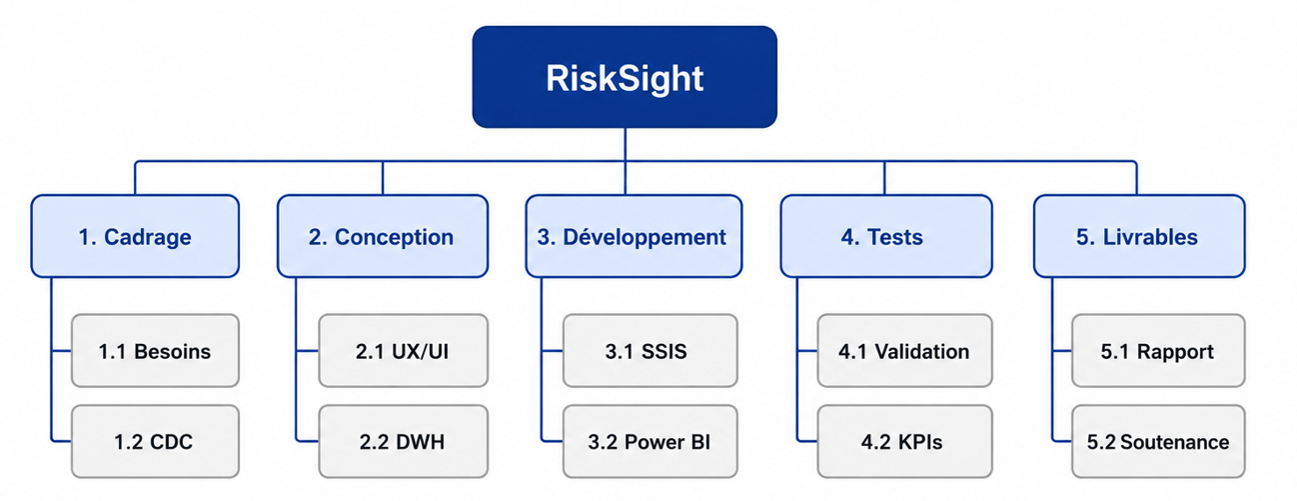
\includegraphics[width=\textwidth]{figures/wbs_risksight.png}

\caption{WBS (Work Breakdown Structure) du projet RiskSight}
\label{fig:wbs}

\end{figure}






\subsection{Livrables et Critères d'Acceptation}

\begin{table}[H]
\centering
\caption{Livrables du projet avec critères d'acceptation mesurables}
\label{tab:livrables}
\renewcommand{\arraystretch}{1.4}
\begin{tabularx}{\textwidth}{p{5cm} p{1.5cm} X p{3cm}}
\toprule
\rowcolor{primary!12}
Livrable & Échéance & Critère d'acceptation & Responsable \\
\midrule
Pipeline SSIS (.dtsx)
  & S4
  & 1\,000 lignes chargées sans erreur en $<$5~min ; 300 dans log\_defauts
  & Rania \\
Data Warehouse SQL Server
  & S4
  & 5 tables + log créées ; clés étrangères validées ; 0 violation FK
  & Rania \\
Dashboard Power BI (3~pages)
  & S6
  & Taux de défaut affiché = 30\% ; PREVIOUSYEAR fonctionnel ; accessible via URL
  & Imane \\
Implémentation Power Query
  & S6
  & Résultats identiques à SSIS ; 1\,000 lignes dans le modèle interne Power BI
  & Imane \\
Rapport technique final
  & S8
  & Chapitres 1--3 complets ; captures d'écran de chaque étape ; bibliographie
  & Binôme \\
Soutenance orale + démo live
  & S8
  & Démonstration du pipeline F5 en direct ; dashboard accessible via URL projetée
  & Binôme \\
\bottomrule
\end{tabularx}
\end{table}






\section{Conclusion}

Ce premier chapitre a pos\'e les bases conceptuelles et entrepreneuriales du
projet RiskSight. L'\'etude de l'existant a mis en \'evidence un vide de march\'e
document\'e, les analyses SWOT, PESTEL et Porter ont confirm\'e la pertinence
strat\'egique de notre solution, et l'\'etude de faisabilit\'e a d\'emontr\'e sa
viabilit\'e \'economique d\`es le troisi\`eme client. Le chapitre suivant
d\'etaillera l'architecture technique et la conception du syst\`eme d'information.

% ============================================================
%  CHAPITRE 2
% ============================================================
\chapter{Analyse et Conception}

\section{Introduction}

Ce chapitre pr\'esente l'architecture technique de RiskSight. Nous y d\'ecrivons
la source de donn\'ees, la mod\'elisation du Data Warehouse en sch\'ema en
\'etoile, la conception du pipeline ETL SSIS et les sp\'ecifications du dashboard
Power~BI.

Ce chapitre présente la mise en oeuvre concrète de RiskSight, de la création du Data Warehouse jusqu'aux résultats visuels du dashboard. Pour chaque étape, nous combinons captures d'écran annotées et explications techniques afin de documenter fidèlement l'implémentation réalisée. Deux méthodes ETL complémentaires sont présentées~: le pipeline SSIS pour une architecture de production robuste, et Power Query pour un prototypage rapide directement dans Power~BI. et ses adaptations au contexte marocain, puis nous décrivons la modélisation du Data Warehouse en schéma en étoile sous SQL~Server 2022, avec ses cinq dimensions et sa table de faits centrale. Nous spécifions ensuite le pipeline ETL SSIS et son alternative Power Query, avant de présenter les trois pages du dashboard Power~BI avec leurs mesures DAX., analysons l'existant concurrentiel via les outils SWOT, PESTEL et Porter, et démontrons la viabilité économique de notre solution par une étude de faisabilité complète. Ces analyses fondent et justifient les choix techniques et architecturaux présentés dans les chapitres suivants.

% -----------------------------------------------------------
\section{Pr\'esentation du Dataset}
% -----------------------------------------------------------

\subsection{Source et Origine des Donn\'ees}

Le jeu de donn\'ees utilis\'e est une adaptation p\'edagogique du
\textit{German Credit Dataset} de l'UCI Machine Learning
Repository~\cite{hofmann1994}. Les adaptations r\'ealis\'ees pour le contexte
Atlas Credit Bank sont~\cite{cdc_atlas}~:

\begin{itemize}
  \item Conversion des montants en Dirhams marocains (1~DM~=~3,5~DH)~;
  \item G\'en\'eration de dates sur la p\'eriode 2020--2024~;
  \item Recodage des variables en libell\'es m\'etier francophones~;
  \item Enrichissement par des variables calcul\'ees (tranches, rangs, m\'edianes)~;
  \item Cr\'eation d'identifiants clients fictifs au format \texttt{ACB-XXXXXX}.
\end{itemize}

\subsection{Caract\'eristiques du Dataset Final}

\begin{table}[H]
\centering
\caption{Caract\'eristiques du fichier \texttt{atlas\_credit\_bank\_2020\_2024.csv}~\cite{cdc_atlas}}
\label{tab:dataset}
\renewcommand{\arraystretch}{1.3}
\begin{tabularx}{\textwidth}{>{\bfseries}p{5cm} X}
\toprule
\rowcolor{primary!12}
Caract\'eristique & Valeur \\
\midrule
Nombre de lignes           & 1\,000 demandes de cr\'edit \\
Nombre de colonnes         & 28 colonnes (apr\`es nettoyage et enrichissement) \\
P\'eriode couverte         & Janvier 2020 --- D\'ecembre 2024 \\
Plage des montants         & 900~DH \`a 64\,500~DH (moyenne~: 11\,451~DH) \\
Taux de d\'efaut           & 30\% (300 d\'efauts / 700 bons clients) \\
Variable cible             & \texttt{defaut} (0 = bon client, 1 = d\'efaut) \\
Encodage                   & UTF-8 BOM (compatible Excel, SSIS, Power~BI) \\
\bottomrule
\end{tabularx}
\end{table}

% -----------------------------------------------------------
\section{Architecture Technique Globale}
% -----------------------------------------------------------

\begin{figure}[H]
\centering
\begin{tikzpicture}[
  layer/.style={rectangle,rounded corners=6pt,draw=primary,fill=primary!10,
                text width=3cm,align=center,minimum height=2.4cm,
                font=\small\bfseries,drop shadow},
  sub/.style={font=\scriptsize,text=darkgray,align=center,text width=3cm},
  arr/.style={-Stealth,very thick,color=secondary,line width=2pt}
]
  \node[layer] (src) {Source\\CSV};
  \node[sub,below=0.15cm of src]{1\,000 lignes\\28 colonnes\\UTF-8 BOM};

  \node[layer,right=1.4cm of src] (etl) {ETL\\SSIS};
  \node[sub,below=0.15cm of etl]{Visual Studio 2022\\Pipeline .dtsx\\2~t\^aches};

  \node[layer,right=1.4cm of etl] (dwh) {Data Warehouse\\SQL Server};
  \node[sub,below=0.15cm of dwh]{Sch\'ema \'etoile\\5~tables + log\\SQL Server 2022};

  \node[layer,right=1.4cm of dwh] (pbi) {Dashboard\\Power BI};
  \node[sub,below=0.15cm of pbi]{3~pages\\Mesures DAX\\Power BI Service};

  \draw[arr] (src)--(etl);
  \draw[arr] (etl)--(dwh);
  \draw[arr] (dwh)--(pbi);
\end{tikzpicture}
\caption{Architecture BI end-to-end de RiskSight~\cite{cdc_atlas}}
\label{fig:architecture}
\end{figure}

\begin{table}[H]
\centering
\caption{Stack technologique du projet~\cite{cdc_atlas}}
\label{tab:stack}
\renewcommand{\arraystretch}{1.3}
\begin{tabularx}{\textwidth}{>{\bfseries}p{4cm} p{4.9cm} X}
\toprule
\rowcolor{primary!12}
Couche & Outil & R\^ole \\
\midrule
Source         & CSV (UTF-8 BOM)        & Donn\'ees brutes adapt\'ees \\
ETL (m\'ethode 1) & SSIS (Visual Studio 2022) & Extraction, transformation, chargement \\
ETL (m\'ethode 2) & Power Query (Power BI Desktop) & Transformation alternative et validation \\
Data Warehouse & SQL Server 2022 Express & Stockage sch\'ema en \'etoile (5~tables) \\
Administration & SSMS                   & Gestion et v\'erification des tables \\
Visualisation  & Power BI Desktop        & Mod\'elisation DAX et dashboard \\
Versioning     & GitHub (repo priv\'e)   & Collaboration et historique \\
\bottomrule
\end{tabularx}
\end{table}

\begin{figure}[H]
\centering
\begin{tabular}{ccc}
\begin{tcolorbox}[mybox,width=4.5cm,height=4.5cm,halign=center,valign=center]
\centering

\includegraphics[height=1.8cm]{figures/sqlserver_logo}\\[0.3cm]
\textbf{SQL Server 2022}\\
\scriptsize\textit{Data Warehouse}
\end{tcolorbox}
&
\begin{tcolorbox}[mybox,width=4.5cm,height=4.5cm,halign=center,valign=center]
\centering

\includegraphics[height=1.8cm]{figures/powerbi_logo}\\[0.3cm]
\textbf{Power BI}\\
\scriptsize\textit{Dashboard \& DAX}
\end{tcolorbox}
&
\begin{tcolorbox}[mybox,width=4.5cm,height=4.5cm,halign=center,valign=center]
\centering

\includegraphics[height=1.8cm]{figures/visualstudio_logo}\\[0.3cm]
\textbf{Visual Studio 2022}\\
\scriptsize\textit{Pipeline SSIS}
\end{tcolorbox}
\\[0.3cm]
\begin{tcolorbox}[mybox,width=4.5cm,height=4.5cm,halign=center,valign=center]
\centering

\includegraphics[height=1.8cm]{figures/python_logo}\\[0.3cm]
\textbf{Python 3.x}\\
\scriptsize\textit{Pré-traitement CSV}
\end{tcolorbox}
&
\begin{tcolorbox}[mybox,width=4.5cm,height=4.5cm,halign=center,valign=center]
\centering

\includegraphics[height=1.8cm]{figures/github}\\[0.3cm]
\textbf{GitHub}\\
\scriptsize\textit{Versioning}
\end{tcolorbox}
&
\begin{tcolorbox}[mybox,width=4.5cm,height=4.5cm,halign=center,valign=center]
\centering

\includegraphics[height=1.8cm]{figures/excel_logo}\\[0.3cm]
\textbf{Microsoft Excel}\\
\scriptsize\textit{Source de données}
\end{tcolorbox}
\end{tabular}
\caption{Stack technologique de RiskSight}
\label{fig:stack_logos}
\end{figure}

\vspace*{1.5cm}% -----------------------------------------------------------
\section{Mod\'elisation du Data Warehouse --- Sch\'ema en \'Etoile}
% -----------------------------------------------------------

\subsection{Principes de la Mod\'elisation Dimensionnelle}

La mod\'elisation dimensionnelle, introduite par Kimball~\cite{kimball}, organise
les donn\'ees en une \textbf{table de faits centrale} entour\'ee de
\textbf{tables de dimensions}. Ce sch\'ema en \'etoile optimise les requ\^etes
analytiques et facilite la compr\'ehension par les utilisateurs m\'etier.

\subsection{Diagramme du Sch\'ema en \'Etoile}

\begin{figure}[H]
\centering
\begin{tikzpicture}[
  fact/.style={rectangle,draw=secondary,fill=secondary!12,rounded corners=4pt,
               text width=4.6cm,align=center,font=\small\bfseries,
               minimum height=3cm,drop shadow},
  dim/.style={rectangle,draw=primary,fill=primary!10,rounded corners=4pt,
              text width=3.4cm,align=center,font=\small,minimum height=2.4cm,
              drop shadow},
  dt/.style={font=\small\bfseries\color{primary}},
  fk/.style={-Stealth,thick,color=primary,dashed}
]
  \node[fact] (fait) at (0,0) {
    \textcolor{secondary}{\textbf{fait\_demande\_credit}}\\[4pt]
    \scriptsize
    id\_fait (PK)\\id\_client (FK)\\id\_temps (FK)\\
    id\_credit (FK)\\id\_profil (FK)\\
    montant\_credit\_dh\\duree\_credit\_mois\\
    \textbf{defaut (0/1)}
  };
  \node[dim] at (-5.5,3) (dc) {
    {\textbf{\textcolor{primary}{dim\_client}}}\\[3pt]\scriptsize
    id\_client (PK)\\age\_client\\tranche\_age\\
    genre / statut\_marital\\niveau\_emploi\\type\_logement
  };
  \node[dim] at (5.5,3) (dt) {
    {\textbf{\textcolor{primary}{dim\_temps}}}\\[3pt]\scriptsize
    id\_temps (PK)\\date\_demande\\
    annee / trimestre\\mois / nom\_mois
  };
  \node[dim] at (-5.5,-3.5) (dcr) {
    {\textbf{\textcolor{primary}{dim\_credit}}}\\[3pt]\scriptsize
    id\_credit (PK)\\objet\_credit\\
    montant / tranche\\duree\_credit\_mois\\charge\_remboursement
  };
  \node[dim] at (5.5,-3.5) (dp) {
   {\textbf{\textcolor{primary}{dim\_profil\_financier}}}\\[3pt]\scriptsize
    id\_profil (PK)\\statut\_compte\_bancaire\\
    niveau\_epargne\\historique\_credit\\type\_propriete
  };
  \draw[fk] (dc)--(fait); \draw[fk] (dt)--(fait);
  \draw[fk] (dcr)--(fait); \draw[fk] (dp)--(fait);
\end{tikzpicture}
\caption{Sch\'ema en \'etoile du Data Warehouse AtlasCreditBank~\cite{cdc_atlas,kimball}}
\label{fig:schema_etoile}
\end{figure}

\vspace*{1.5cm}
\subsection{Description des Tables}

Le schéma en étoile du Data Warehouse AtlasCreditBank comprend six tables~\cite{cdc_atlas}~:

\begin{itemize}
  \item \textbf{fait\_demande\_credit}~: table centrale contenant 1\,000~lignes. Elle enregistre chaque demande de crédit avec les clés étrangères vers les quatre dimensions et les mesures quantitatives (montant, durée, mensualité, défaut)~;
  \item \textbf{dim\_client}~: 1\,000~lignes décrivant le profil sociodémographique de chaque emprunteur (âge, genre, statut marital, niveau d'emploi, type de logement)~;
  \item \textbf{dim\_temps}~: 1\,000~lignes représentant les dates de demande avec décomposition en année, trimestre, mois et nom du mois pour faciliter l'analyse temporelle~;
  \item \textbf{dim\_credit}~: 1\,000~lignes décrivant les caractéristiques de chaque crédit (objet, montant, tranche, durée, charge de remboursement)~;
  \item \textbf{dim\_profil\_financier}~: 1\,000~lignes contenant le profil financier de l'emprunteur (statut du compte bancaire, niveau d'épargne, historique crédit, type de propriété)~;
  \item \textbf{log\_defauts}~: 300~lignes enregistrant uniquement les clients en défaut, utilisée pour le suivi et l'audit du risque crédit.
\end{itemize}, dim\_client, dim\_temps,
dim\_credit, dim\_profil\_financier, log\_defauts) avec leur r\^ole, leur
cardinal et leurs colonnes principales. R\'ef\'erencez \cite{cdc_atlas}.]

% -----------------------------------------------------------
\section{Conception du Pipeline ETL SSIS}
% -----------------------------------------------------------

\subsection{Vue d'Ensemble du Pipeline}

\begin{figure}[H]
\centering
\begin{tikzpicture}[
  comp/.style={rectangle,rounded corners=3pt,draw=primary,fill=primary!10,
               text width=3cm,align=center,minimum height=1cm,font=\small},
  arr/.style={-Stealth,thick,color=primary}
]
  \node[comp] (src)  {Flat File Source\\(CSV UTF-8)};
  \node[comp,below=0.5cm of src]  (dc)   {Data Conversion\\(28 colonnes)};
  \node[comp,below=0.5cm of dc]   (der)  {Derived Column\\(3 col. calcul\'ees)};
  \node[comp,below=0.5cm of der]  (sort) {Sort (date\_demande)};
  \node[comp,below=0.5cm of sort] (cs)   {Conditional Split\\(Sain / D\'efaut)};
  \node[comp,below=0.5cm of cs]   (ua)   {Union All};
  \node[comp,below=0.5cm of ua]   (mc)   {Multicast};

  
% ---------------- Dimensions sous Multicast ----------------

\node[comp,below left=4cm and 1cm of mc] (d1)
  {dest.\\dim\_client};

\node[comp,below left=2cm and 3cm of mc] (d2)
  {dest.\\dim\_credit};

\node[comp,below=2cm of mc] (d3)
  {dest.\\dim\_temps};

\node[comp,below right=4cm and 1cm of mc] (d4)
  {dest.\\dim\_profil};

\node[comp,below right=2cm and 4cm of mc] (d5)
  {dest.\\log\_defauts};
  
  \draw[arr] (src)--(dc); \draw[arr] (dc)--(der);
  \draw[arr] (der)--(sort); \draw[arr] (sort)--(cs);
  \draw[arr] (cs)--(ua); \draw[arr] (ua)--(mc);
  \draw[arr] (mc)--(d1); \draw[arr] (mc)--(d2);
  \draw[arr] (mc)--(d3); \draw[arr] (mc)--(d4);
  \draw[arr] (mc)--(d5);
\end{tikzpicture}



\caption{Flux de donn\'ees de la T\^ache~1 SSIS --- Chargement des dimensions~\cite{guide_etl}}
\label{fig:ssis_task1}
\end{figure}

\subsection{Composants SSIS Utilis\'es}

\begin{table}[H]
\centering
\caption{Composants SSIS du pipeline ETL~\cite{guide_etl,cdc_atlas}}
\label{tab:ssis_composants}
\renewcommand{\arraystretch}{1.4}
\begin{tabularx}{\textwidth}{p{4cm} p{2.5cm} X}
\toprule
\rowcolor{primary!12}
Composant SSIS & Type & Application dans le projet \\
\midrule
Flat File Source   & Extract   & Lecture du CSV \texttt{atlas\_credit\_bank} \\
Derived Column     & Transform & Calcul mensualit\'e, cat\'egorie risque, ann\'ee naissance \\
Data Conversion    & Transform & Typage~: Date, Integer, SmallInt, Float, NVARCHAR \\
Conditional Split  & Transform & S\'eparation clients sains / clients en d\'efaut \\
Sort               & Transform & Tri par \texttt{date\_demande} pour \texttt{dim\_temps} \\
Multicast          & Load      & Duplication du flux vers les 4~dimensions \\
Lookup             & Load      & R\'ecup\'eration des IDs pour la table de faits \\
OLE DB Destination & Load      & Insertion dans SQL~Server (6~tables) \\
\bottomrule
\end{tabularx}
\end{table}
\vspace*{1cm}
\subsection{Colonnes D\'eriv\'ees Calcul\'ees}

\begin{table}[H]
\centering
\caption{Colonnes d\'eriv\'ees cr\'e\'ees dans le composant \textit{Derived Column}}
\label{tab:derived}
\renewcommand{\arraystretch}{1.3}
\begin{tabularx}{\textwidth}{>{\ttfamily}p{4.8cm} X p{3.5cm}}
\toprule
\rowcolor{primary!12}
Nom de la colonne & Expression SSIS & Type SQL \\
\midrule
mensualite\_estimee\_dh
  & \texttt{(DT\_I4)(montant\_conv / duree\_conv)} & INT \\
categorie\_risque
  & \texttt{defaut\_conv == 1 ? "Client a risque" : "Client sain"}
  & NVARCHAR(50) \\
annee\_naissance
  & \texttt{(DT\_I2)(2024 - age\_conv)} & SMALLINT \\
\bottomrule
\end{tabularx}
\end{table}
\vspace*{1.5cm}

\newpage
% -----------------------------------------------------------
\section{Sp\'ecification du Dashboard Power BI}
% -----------------------------------------------------------

\subsection{Page 1 --- Vue Executive (KPIs Globaux)}

\textbf{Destinataire~:} Direction G\'en\'erale.
\textbf{Question m\'etier~:} Comment se porte le portefeuille cr\'edit globalement~?~\cite{cdc_atlas}

\begin{itemize}
  \item KPI~: Taux de d\'efaut global (30\%)
  \item KPI~: Volume total de cr\'edits accord\'es en DH
  \item KPI~: Nombre de demandes trait\'ees
  \item KPI~: Montant moyen par cr\'edit
  \item Courbe~: \'Evolution du taux de d\'efaut par ann\'ee (2020--2024)
  \item Treemap~: R\'epartition des demandes par objet de cr\'edit
\end{itemize}

\vspace*{1cm}
\subsection{Page 2 --- Analyse du Risque par Profil}

\textbf{Destinataire~:} D\'epartement Risques.
\textbf{Question m\'etier~:} Qui sont les clients les plus risqu\'es~?

\begin{itemize}
  \item Barres~: Taux de d\'efaut par statut du compte bancaire
  \item Barres~: Taux de d\'efaut par historique de cr\'edit (variable la plus pr\'edictive)
  \item Barres~: Taux de d\'efaut par niveau d'\'epargne (ordonn\'e par rang)
  \item Barres group\'ees~: Taux de d\'efaut par tranche d'\^age
  \item Matrice~: Croisement montant $\times$ dur\'ee du cr\'edit
\end{itemize}
\vspace*{1cm}

\subsection{Page 3 --- Analyse Temporelle}

\textbf{Destinataire~:} Direction Risques et Marketing.
\textbf{Question m\'etier~:} Quand le risque est-il le plus \'elev\'e~?

\begin{itemize}
  \item Courbe~: Volume de demandes par mois (saisonnalit\'e)
  \item Barres~: Taux de d\'efaut par trimestre (T1 \`a T4)
  \item Courbe~: \'Evolution du montant moyen par ann\'ee
  \item Comparaison~: Taux de d\'efaut ann\'ee N vs N-1 (mesure DAX \texttt{PREVIOUSYEAR})
\end{itemize}

\subsection{Mesures DAX Principales}

\begin{table}[H]
\centering
\caption{Mesures DAX du mod\`ele Power~BI~\cite{cdc_atlas,ferrari_dax}}
\label{tab:dax}
\renewcommand{\arraystretch}{1.4}
\begin{tabularx}{\textwidth}{>{\ttfamily\bfseries}p{4.8cm} X}
\toprule
\rowcolor{primary!12}
Nom de la mesure & Formule DAX \\
\midrule
Taux\_Defaut      & \texttt{AVERAGE(fait\_demande\_credit[defaut])} \\
Nb\_Defauts       & \texttt{SUM(fait\_demande\_credit[defaut])} \\
Volume\_Total\_DH & \texttt{SUM(fait\_demande\_credit[montant\_credit\_dh])} \\
Montant\_Moyen\_DH & \texttt{AVERAGE(fait\_demande\_credit[montant\_credit\_dh])} \\
Taux\_Defaut\_PY  & \texttt{CALCULATE([Taux\_Defaut], PREVIOUSYEAR(dim\_temps[date\_demande]))} \\
Variation\_Defaut & \texttt{[Taux\_Defaut] - [Taux\_Defaut\_PY]} \\
\bottomrule
\end{tabularx}
\end{table}

\section{Conclusion}

Ce chapitre a pr\'esent\'e l'ensemble de la conception technique de RiskSight~:
mod\'elisation du Data Warehouse en sch\'ema en \'etoile, architecture du pipeline
ETL SSIS en deux t\^aches s\'equentielles et sp\'ecification du dashboard Power~BI
en trois pages. Le chapitre suivant d\'etaillera la phase de r\'ealisation avec
les captures d'\'ecran et les r\'esultats obtenus.

% ============================================================
%  CHAPITRE 3
% ============================================================
\chapter{R\'ealisation}

\section{Introduction}

Ce chapitre pr\'esente la mise en \oe uvre concr\`ete de l'architecture RiskSight.
Nous d\'ecrivons successivement la cr\'eation du Data Warehouse, l'impl\'ementation
du pipeline SSIS (premi\`ere m\'ethode ETL), l'impl\'ementation via Power Query
(seconde m\'ethode ETL) et les r\'esultats du dashboard Power~BI.

Ce chapitre détaille l'architecture technique de RiskSight. Nous présentons d'abord le dataset source et ses adaptations au contexte marocain, puis nous décrivons la modélisation du Data Warehouse en schéma en étoile sous SQL~Server 2022, avec ses cinq dimensions et sa table de faits centrale. Nous spécifions ensuite le pipeline ETL SSIS et son alternative Power Query, avant de présenter les trois pages du dashboard Power~BI avec leurs mesures DAX.

% -----------------------------------------------------------
\section{Cr\'eation du Data Warehouse sous SQL~Server}
% -----------------------------------------------------------

\subsection{Cr\'eation de la Base de Donn\'ees}

La base de données \texttt{AtlasCreditBank} a été créée dans SQL~Server Management Studio (SSMS) en exécutant le script de création via \texttt{Nouvelle requête}. Après exécution du script complet (cf. Annexe~A), SSMS affiche les six tables du schéma \texttt{atlas\_dwh} dans l'explorateur d'objets, confirmant la création correcte de la structure du Data Warehouse. dans SSMS.
Ins\'erez une capture d'\'ecran de SSMS montrant la base de donn\'ees cr\'e\'ee.]

\begin{figure}[H]
\centering
\fbox{\parbox{13cm}{\centering\vspace{2cm}
  [Capture d'\'ecran SSMS --- Vue des 6~tables dans atlas\_dwh]\\
  Ajoutez votre image : \texttt{figures/ssms\_tables.png}\\
  Commande : \texttt{\textbackslash includegraphics[width=13cm]\{figures/ssms\_tables\}}
  \vspace{2cm}}}
\caption{Vue des 6~tables du Data Warehouse dans SSMS}
\label{fig:ssms_tables}
\end{figure}

\begin{lstlisting}[language=SQL, caption={Script de cr\'eation du sch\'ema et des 6~tables~\cite{guide_etl}},
  label={lst:create_tables}]
CREATE SCHEMA atlas_dwh;
GO

CREATE TABLE atlas_dwh.dim_temps (
    id_temps      INT IDENTITY(1,1) PRIMARY KEY,
    date_demande  DATE         NOT NULL,
    annee         SMALLINT     NOT NULL,
    trimestre     NVARCHAR(5)  NOT NULL,
    mois          SMALLINT     NOT NULL,
    nom_mois      NVARCHAR(20) NOT NULL
);

CREATE TABLE atlas_dwh.dim_client (
    id_client              NVARCHAR(50) PRIMARY KEY,
    age_client             INT          NOT NULL,
    tranche_age            NVARCHAR(50) NOT NULL,
    genre                  NVARCHAR(50) NOT NULL,
    statut_marital         NVARCHAR(50) NOT NULL,
    niveau_emploi          NVARCHAR(50) NOT NULL,
    anciennete_emploi      NVARCHAR(50) NOT NULL,
    rang_anciennete        SMALLINT     NOT NULL,
    anciennete_mediane_ans FLOAT        NOT NULL,
    annee_naissance        SMALLINT     NOT NULL,
    type_logement          NVARCHAR(50) NOT NULL
);

CREATE TABLE atlas_dwh.dim_credit (
    id_credit              INT IDENTITY(1,1) PRIMARY KEY,
    objet_credit           NVARCHAR(50) NOT NULL,
    montant_credit_dh      INT          NOT NULL,
    tranche_montant_dh     NVARCHAR(50) NOT NULL,
    duree_credit_mois      INT          NOT NULL,
    mensualite_estimee_dh  INT          NOT NULL,
    charge_remboursement   NVARCHAR(50) NOT NULL,
    rang_charge            SMALLINT     NOT NULL,
    a_garant               NVARCHAR(50) NOT NULL,
    autres_credits_en_cours NVARCHAR(50) NOT NULL
);

CREATE TABLE atlas_dwh.dim_profil_financier (
    id_profil              INT IDENTITY(1,1) PRIMARY KEY,
    statut_compte_bancaire NVARCHAR(50) NOT NULL,
    niveau_epargne         NVARCHAR(50) NOT NULL,
    historique_credit      NVARCHAR(50) NOT NULL,
    type_propriete         NVARCHAR(50) NOT NULL
);

CREATE TABLE atlas_dwh.fait_demande_credit (
    id_fait               INT IDENTITY(1,1) PRIMARY KEY,
    id_client             NVARCHAR(50) NOT NULL
        REFERENCES atlas_dwh.dim_client(id_client),
    id_temps              INT NOT NULL
        REFERENCES atlas_dwh.dim_temps(id_temps),
    id_credit             INT NOT NULL
        REFERENCES atlas_dwh.dim_credit(id_credit),
    id_profil             INT NOT NULL
        REFERENCES atlas_dwh.dim_profil_financier(id_profil),
    montant_credit_dh     INT      NOT NULL,
    duree_credit_mois     INT      NOT NULL,
    mensualite_estimee_dh INT      NOT NULL,
    rang_charge           SMALLINT NOT NULL,
    anciennete_mediane_ans FLOAT   NOT NULL,
    defaut                SMALLINT NOT NULL
);

CREATE TABLE atlas_dwh.log_defauts (
    id_log            INT IDENTITY(1,1) PRIMARY KEY,
    id_client         NVARCHAR(50) NOT NULL,
    date_demande      DATETIME     NOT NULL,
    montant_credit_dh INT          NOT NULL,
    categorie_risque  NVARCHAR(50) NOT NULL
);
\end{lstlisting}

% -----------------------------------------------------------
\section{Impl\'ementation du Pipeline ETL avec SSIS}
% -----------------------------------------------------------

\subsection{Configuration des Connexions}

Deux connexions sont configurées dans le Connection Manager de Visual Studio 2022. La source CSV utilise un \textbf{Flat File Connection Manager} paramétré en UTF-8 (code page 65001) avec le point-virgule comme délimiteur. La destination SQL~Server utilise un \textbf{OLE~DB Connection Manager} pointant vers l'instance locale \texttt{.\\SQLEXPRESS}, base de données \texttt{AtlasCreditBank}. (code page 65001 UTF-8)
et SQL~Server OLE~DB. Ins\'erez une capture d'\'ecran de la fen\^etre de
configuration de Visual Studio 2022.]

\begin{figure}[H]
\centering
\fbox{\parbox{13cm}{\centering\vspace{2cm}
  [Capture d'\'ecran --- Connection Managers SSIS]\\
  \texttt{figures/ssis\_connections.png}
  \vspace{2cm}}}
\caption{Configuration des connexions dans SSIS (Visual Studio 2022)}
\label{fig:ssis_connections}
\end{figure}

\subsection{T\^ache 1 --- Chargement des Dimensions}

[D\'ecrivez chaque composant de la T\^ache~1~: Flat File Source, Data Conversion,
Derived Column, Sort, Conditional Split, Union All, Multicast, et les
5~destinations OLE~DB. Ins\'erez les captures d'\'ecran du canvas SSIS.]

\begin{figure}[H]
\centering
\fbox{\parbox{13cm}{\centering\vspace{2.5cm}
  [Capture d'\'ecran --- Canvas SSIS T\^ache~1]\\
  \texttt{figures/ssis\_task1\_canvas.png}
  \vspace{2.5cm}}}
\caption{Canvas de la T\^ache~1 SSIS --- Chargement des dimensions~\cite{guide_etl}}
\label{fig:ssis_task1_canvas}
\end{figure}

\subsection{T\^ache 2 --- Chargement de la Table de Faits}

\begin{tcolorbox}[warningbox,title={Point critique --- T\^ache s\'equentielle}]
La table de faits doit \^etre charg\'ee dans une \textbf{deuxi\`eme t\^ache
s\'epar\'ee}, connect\'ee \`a la premi\`ere par une contrainte de pr\'ec\'edence
(fl\`eche verte) dans le Control Flow. Les Lookups \'echouent si les dimensions
sont vides au moment de leur ex\'ecution~\cite{guide_etl}.
\end{tcolorbox}

\begin{table}[H]
\centering
\caption{Configuration des 4~Lookups de la T\^ache~2~\cite{guide_etl}}
\label{tab:lookups}
\renewcommand{\arraystretch}{1.4}
\begin{tabularx}{\textwidth}{p{3.5cm} p{4cm} X}
\toprule
\rowcolor{primary!12}
Lookup & Table de r\'ef\'erence & Colonne r\'ecup\'er\'ee \\
\midrule
Recherche Client
  & atlas\_dwh.dim\_client
  & id\_client\_lkp \\
Recherche Temps
  & atlas\_dwh.dim\_temps
  & id\_temps\_lkp \\
Recherche Cr\'edit
  & atlas\_dwh.dim\_credit
  & id\_credit\_lkp \\
Recherche Profil
  & atlas\_dwh.dim\_profil\_financier
  & id\_profil\_lkp \\
\bottomrule
\end{tabularx}
\end{table}

\subsection{V\'erification par Requ\^ete SQL}

\begin{lstlisting}[language=SQL, caption={Requ\^ete de v\'erification apr\`es ex\'ecution~\cite{guide_etl}},
  label={lst:verification}]
SELECT 'dim_client'            AS table_name, COUNT(*) AS nb_lignes
  FROM atlas_dwh.dim_client
UNION ALL SELECT 'dim_temps',            COUNT(*) FROM atlas_dwh.dim_temps
UNION ALL SELECT 'dim_credit',           COUNT(*) FROM atlas_dwh.dim_credit
UNION ALL SELECT 'dim_profil_financier', COUNT(*) FROM atlas_dwh.dim_profil_financier
UNION ALL SELECT 'fait_demande_credit',  COUNT(*) FROM atlas_dwh.fait_demande_credit
UNION ALL SELECT 'log_defauts',          COUNT(*) FROM atlas_dwh.log_defauts;
\end{lstlisting}

\begin{table}[H]
\centering
\caption{R\'esultats attendus apr\`es ex\'ecution du pipeline SSIS~\cite{guide_etl}}
\label{tab:resultats_ssis}
\begin{tabular}{lc}
\toprule
\rowcolor{primary!12}
Table & Lignes attendues \\
\midrule
dim\_client              & 1\,000 \\
dim\_temps               & 1\,000 \\
dim\_credit              & 1\,000 \\
dim\_profil\_financier   & 1\,000 \\
fait\_demande\_credit    & 1\,000 \\
log\_defauts             & 300 \\
\bottomrule
\end{tabular}
\end{table}

% -----------------------------------------------------------
\section{Impl\'ementation ETL avec Power Query (2\textsuperscript{e} M\'ethode)}
% -----------------------------------------------------------

\begin{tcolorbox}[mybox,title={Pourquoi une deuxi\`eme m\'ethode ETL~?}]
Afin de d\'emontrer la ma\^itrise de plusieurs outils de la cha\^ine BI et de
valider les r\'esultats obtenus par SSIS, nous avons \'egalement impl\'ement\'e
le pipeline d'extraction et de transformation directement dans
\textbf{Power Query} (\'editeur int\'egr\'e \`a Power~BI Desktop). Les deux
impl\'ementations produisent des r\'esultats identiques, ce qui atteste de la
robustesse de notre approche.
\end{tcolorbox}

\subsection{Connexion et Transformations dans Power Query}

[D\'ecrivez les \'etapes de connexion au fichier CSV dans Power~BI Desktop
et les transformations appliqu\'ees~: typage des colonnes, colonnes calcul\'ees,
gestion des valeurs nulles. Ins\'erez les captures d'\'ecran.]

\begin{figure}[H]
\centering
\fbox{\parbox{13cm}{\centering\vspace{2cm}
  [Capture d'\'ecran --- \'Editeur Power Query]\\
  \texttt{figures/powerquery\_steps.png}
  \vspace{2cm}}}
\caption{\'Etapes de transformation dans Power Query}
\label{fig:pq_steps}
\end{figure}

\subsection{Comparaison SSIS vs Power Query}

\begin{table}[H]
\centering
\caption{Comparaison des deux approches ETL}
\label{tab:ssis_vs_pq}
\renewcommand{\arraystretch}{1.4}
\begin{tabularx}{\textwidth}{>{\bfseries}p{5cm} X X}
\toprule
\rowcolor{primary!12}
Crit\`ere & SSIS & Power Query \\
\midrule
Environnement       & Visual Studio 2022 & Power~BI Desktop \\
Type de d\'eveloppement & Visuel + configuration & Visuel + langage M \\
Cible de chargement & SQL~Server (DWH) & Mod\`ele interne Power~BI \\
Gestion des erreurs & Contraintes FK, logs d\'edi\'es & Moins fin \\
Scalabilit\'e       & Tr\`es \'elev\'ee (millions lignes) & Correcte (dizaines de milliers) \\
Courbe d'apprentissage & \'Elev\'ee & Mod\'er\'ee \\
Cas d'usage optimal & Production, volumes importants & Prototypage rapide, PME \\
\bottomrule
\end{tabularx}
\end{table}
\newpage
% -----------------------------------------------------------
\section{Dashboard Power BI --- R\'esultats Obtenus}
% -----------------------------------------------------------

\subsection{Page 1 --- Vue Executive}

\begin{figure}[H]
\centering
\fbox{\parbox{13cm}{\centering\vspace{3cm}
  [Capture d'\'ecran --- Page~1 Power~BI~: Vue Executive]\\
  \texttt{figures/pbi\_page1\_executive.png}
  \vspace{3cm}}}
\caption{Page~1 du Dashboard RiskSight --- Vue Executive (KPIs globaux)}
\label{fig:pbi_page1}
\end{figure}

[Commentez les r\'esultats affich\'es~: taux de d\'efaut global (30\%),
volume total des cr\'edits, nombre de demandes, montant moyen, \'evolution
2020--2024.]

\subsection{Page 2 --- Analyse du Risque par Profil}

\begin{figure}[H]
\centering
\fbox{\parbox{13cm}{\centering\vspace{3cm}
  [Capture d'\'ecran --- Page~2 Power~BI~: Analyse du Risque]\\
  \texttt{figures/pbi\_page2\_risque.png}
  \vspace{3cm}}}
\caption{Page~2 du Dashboard RiskSight --- Analyse du risque par profil client}
\label{fig:pbi_page2}
\end{figure}

[Commentez les principaux enseignements~: quel statut de compte pr\'esente
le plus fort taux de d\'efaut~? Quel historique cr\'edit est le plus pr\'edictif~?]

\subsection{Page 3 --- Analyse Temporelle}

\begin{figure}[H]
\centering
\fbox{\parbox{13cm}{\centering\vspace{3cm}
  [Capture d'\'ecran --- Page~3 Power~BI~: Analyse Temporelle]\\
  \texttt{figures/pbi\_page3\_temps.png}
  \vspace{3cm}}}
\caption{Page~3 du Dashboard RiskSight --- Analyse temporelle du risque cr\'edit}
\label{fig:pbi_page3}
\end{figure}

[Commentez les r\'esultats temporels~: saisonnalit\'e, trimestre le plus risqu\'e,
comparaison N vs N-1 via la mesure DAX \texttt{PREVIOUSYEAR}.]

% -----------------------------------------------------------
\section{Erreurs Rencontr\'ees et Solutions Apport\'ees}
% -----------------------------------------------------------

\begin{table}[H]
\centering
\caption{Principales erreurs rencontr\'ees et solutions~\cite{guide_etl}}
\label{tab:erreurs}
\renewcommand{\arraystretch}{1.4}
\begin{tabularx}{\textwidth}{p{5.5cm} p{4cm} X}
\toprule
\rowcolor{primary!12}
Erreur & Cause & Solution \\
\midrule
\textit{Cannot convert between unicode and non-unicode}
  & Type VARCHAR au lieu de NVARCHAR
  & \texttt{ALTER TABLE ... ALTER COLUMN ... NVARCHAR(50)} \\
\textit{Truncation may occur}
  & Longueur de colonne trop petite
  & Augmenter \`a NVARCHAR(50) \\
\textit{Violation de cl\'e primaire}
  & Tables non vid\'ees avant re-ex\'ecution
  & Script DELETE + RESEED avant F5 \\
\textit{fait\_demande\_credit = 0 lignes}
  & Lookups ex\'ecut\'es avant le chargement des dimensions
  & S\'eparer en 2~t\^aches s\'equentielles \\
\textit{Row yielded no match during lookup}
  & Table de r\'ef\'erence vide au moment du Lookup
  & V\'erifier la s\'equence Control Flow \\
\bottomrule
\end{tabularx}
\end{table}
\vspace*{1.5cm}
\section{Conclusion}

Ce chapitre a pr\'esent\'e la r\'ealisation compl\`ete du projet RiskSight~:
cr\'eation du Data Warehouse sous SQL~Server, pipeline ETL SSIS fonctionnel
(1\,000~lignes charg\'ees dans chaque table de dimension, 300~dans log\_defauts),
impl\'ementation alternative via Power Query, et dashboard Power~BI en
trois pages. Les deux approches ETL produisent des r\'esultats coh\'erents,
ce qui valide la robustesse de l'architecture propos\'ee.

% ============================================================
%  CONCLUSION GENERALE
% ============================================================
\chapter*{Conclusion G\'en\'erale et Perspectives}
\addcontentsline{toc}{chapter}{Conclusion G\'en\'erale et Perspectives}
\markboth{Conclusion G\'en\'erale et Perspectives}{Conclusion G\'en\'erale et Perspectives}

\section*{Bilan du projet}

Ce projet avait pour objectif de répondre à une problématique concrète~: comment automatiser le pilotage du risque crédit pour les institutions financières marocaines, sans expertise IT et à coût accessible~? Pour y répondre, nous avons conçu et développé \textbf{RiskSight}, une plateforme SaaS de scoring et de pilotage du risque crédit reposant sur une architecture Business Intelligence complète \textit{end-to-end}. Le pipeline ETL SSIS extrait, transforme et charge 1\,000~dossiers de crédit dans un Data Warehouse modélisé en schéma en étoile sous SQL~Server 2022. Le dashboard Power~BI en trois pages restitue les indicateurs clés de risque, accessibles via URL sans installation. L'étude de faisabilité entrepreneuriale confirme la viabilité économique du projet~: le seuil de rentabilité est atteint dès 3~clients, avec une marge sur coût variable de 92\% et un résultat net Year~1 estimé à 825\,573~DH pour 19~clients pilotes.~: rappel de la probl\'ematique, r\'esum\'e des
travaux r\'ealis\'es (ETL SSIS, Data Warehouse, dashboard Power~BI), r\'esultats
obtenus et validation de la faisabilit\'e entrepreneuriale.]

\section*{Objectifs atteints}

\begin{itemize}
  \item Pipeline ETL SSIS complet et fonctionnel (1\,000~lignes charg\'ees)~;
  \item Data Warehouse en sch\'ema en \'etoile (5~tables + log)~;
  \item Dashboard Power~BI en 3~pages avec mesures DAX avanc\'ees~;
  \item Impl\'ementation alternative via Power Query (validation crois\'ee)~;
  \item \'Etude de march\'e compl\`ete (SWOT, PESTEL, Porter)~;
  \item Faisabilit\'e \'economique prouv\'ee (SR = 3~clients, marge $\approx$92\%).
\end{itemize}

\section*{Limites et Perspectives}

\subsection*{Limites du prototype actuel}

\begin{itemize}
  \item \textbf{Dataset statique et pédagogique}~: la version actuelle repose sur
    une adaptation du German Credit Dataset, non sur des données réelles de
    microfinances marocaines. Les distributions statistiques ne reflètent pas
    nécessairement le comportement crédit local.
  \item \textbf{Interface d'upload non implémentée}~: le client ne peut pas encore
    déposer son propre fichier CSV. Cette fonctionnalité constitue le premier
    chantier de la V2.
  \item \textbf{Absence de modèle prédictif}~: le tableau de bord affiche des
    indicateurs descriptifs mais n'anticipe pas le risque de défaut futur.
  \item \textbf{Dépendance à l'écosystème Microsoft}~: SQL Server, SSIS et
    Power BI créent une dépendance à un seul éditeur.
\end{itemize}

\subsection*{Perspective 1 --- Module de Scoring par Machine Learning}

La première extension naturelle consiste à intégrer un modèle prédictif de
scoring crédit directement dans le pipeline ETL. Trois algorithmes sont
candidats~\cite{lessmann2015}~:

\begin{table}[H]
\centering
\caption{Algorithmes de scoring crédit envisagés}
\renewcommand{\arraystretch}{1.3}
\begin{tabularx}{\textwidth}{p{4cm} X p{3cm}}
\toprule
\rowcolor{primary!12}
Algorithme & Avantage pour le scoring crédit & AUC typique \\
\midrule
Régression logistique & Interprétable, requis par les régulateurs (BAM) & 0.72--0.76 \\
Random Forest & Robuste aux données déséquilibrées (70/30) & 0.78--0.83 \\
XGBoost & Meilleure performance sur données tabulaires & 0.80--0.86 \\
\bottomrule
\end{tabularx}
\end{table}

Le modèle serait entraîné sur le dataset historique, sérialisé (\texttt{.pkl}),
et exposé comme service REST appelé par Power BI via un connecteur Python.
Chaque nouveau dossier reçoit un \textbf{score de risque de 0 à 100} affiché
dans une nouvelle page du dashboard~\cite{worldbank}.
\vspace{0.4cm}


\subsection*{Perspective 2 --- Architecture Multi-Agents LLM pour l'analyse
  intelligente du risque}

Une évolution plus ambitieuse consiste à remplacer le dashboard statique par
un \textbf{système multi-agents} basé sur des Large Language Models (LLM),
selon le paradigme des \textit{Agentic AI Systems}.

L'architecture proposée comprend trois agents spécialisés~:

\begin{itemize}
  \item \textbf{Agent Ingestion}~: surveille en temps réel les dépôts de fichiers
    CSV clients, déclenche le pipeline ETL automatiquement, valide la qualité des
    données et génère un rapport d'anomalies en langage naturel.
  \item \textbf{Agent Analyse}~: interroge le Data Warehouse via des requêtes SQL
    auto-générées (Text-to-SQL), produit des analyses de risque narratives
    (\textit{``Le taux de défaut a augmenté de 4~points sur T3 2024 --- principalement
    porté par le segment clients sans historique crédit''}), et déclenche des alertes
    automatiques si un KPI franchit un seuil critique.
  \item \textbf{Agent Reporting}~: génère automatiquement un rapport mensuel en PDF
    (résumé exécutif, graphiques, recommandations) directement depuis les données
    du DWH, sans intervention humaine.
\end{itemize}

Ces agents communiquent via un orchestrateur (LangGraph ou AutoGen) et sont
exposés au client via une interface de chat intégrée au dashboard. Le
responsable crédit peut poser des questions en français~:
\textit{``Quels clients ont un risque de défaut supérieur à 70\% ce mois-ci ?''}
et reçoit une réponse structurée en quelques secondes.
\vspace{0.4cm}
\subsection*{Perspective 3 --- Interface d'upload multi-sources et mapping
  intelligent de colonnes}

La V2 commerciale prévoit une interface web complète permettant~:
\begin{itemize}
  \item L'\textbf{upload autonome} de fichiers CSV ou Excel par le client,
    sans intervention de notre équipe~;
  \item Un \textbf{module de mapping intelligent}~: l'interface détecte
    automatiquement les colonnes du fichier client et les aligne sur notre
    schéma standard via un algorithme de similarité sémantique (sentence
    embeddings). Un tableau de correspondance configurable permet au client
    de valider ou corriger les mappings en quelques clics~;
  \item Un \textbf{dashboard multi-tenant}~: chaque institution financière
    dispose de son espace cloisonné, avec authentification OAuth2 et
    données hébergées dans un schéma SQL Server séparé.
  \item Une \textbf{API REST publique}~: permettant aux institutions
    disposant d'un système Core Banking de pousser leurs données
    directement sans passer par un fichier CSV.
\end{itemize}

Ces trois perspectives forment une feuille de route cohérente~: V1
(prototype BI fonctionnel, objet de ce rapport) $\to$ V2 (interface
autonome + scoring ML) $\to$ V3 (système multi-agents LLM + API).

% ============================================================
%  REFERENCES BIBLIOGRAPHIQUES (inline — pas de .bib externe)
% ============================================================
\begin{thebibliography}{99}
\addcontentsline{toc}{chapter}{R\'ef\'erences bibliographiques}

%% ── Dataset ──────────────────────────────────────────────────
\bibitem{hofmann1994}
H.~Hofmann,
\textit{Statlog (German Credit Data)},
UCI Machine Learning Repository, University of Hamburg, 1994.
Disponible~: \url{https://archive.ics.uci.edu/dataset/144/statlog+german+credit+data}
[Dataset adapt\'e pour le contexte marocain Atlas Credit Bank 2020--2024~:
conversion en Dirhams, g\'en\'eration de dates, recodage en libell\'es m\'etier].

%% ── Business Intelligence ────────────────────────────────────
\bibitem{kimball}
R.~Kimball et M.~Ross,
\textit{The Data Warehouse Toolkit: The Definitive Guide to Dimensional
Modeling}, 3\textsuperscript{e}~\'ed.
Wiley, 2013.
ISBN~978-1-118-53080-1.

\bibitem{inmon}
W.~H.~Inmon,
\textit{Building the Data Warehouse}, 4\textsuperscript{e}~\'ed.
Wiley, 2005.
ISBN~978-0-7645-9944-6.

%% ── Power BI & DAX ───────────────────────────────────────────
\bibitem{ferrari_dax}
A.~Ferrari et M.~Russo,
\textit{The Definitive Guide to DAX: Business Intelligence for Microsoft
Power BI, SQL Server Analysis Services, and Excel}, 2\textsuperscript{e}~\'ed.
Microsoft Press, 2019.
ISBN~978-1-5093-0903-6.

%% ── Gestion de projet ────────────────────────────────────────
\bibitem{pmbok}
Project Management Institute,
\textit{A Guide to the Project Management Body of Knowledge (PMBOK Guide)},
7\textsuperscript{e}~\'ed.
PMI, Newtown Square, PA, 2021.
ISBN~978-1-62825-664-2.

\bibitem{cours_gp}
I.~Daoudi, K.~Bousmar, H.~Ouzif et D.~Monsif,
\textit{Cours de Gestion de Projet --- Chapitre~II~: M\'ethodes de gestion
de projet informatique}.
Support de cours, Fili\`ere 4IIR, EMSI, 2025.
[Parties prenantes, cycle de vie, mod\`eles de d\'eveloppement, gestion des co\^uts].

%% ── Strategie & entrepreneuriat ─────────────────────────────
\bibitem{porter}
M.~E.~Porter,
\textit{Competitive Strategy: Techniques for Analyzing Industries and
Competitors}.
Free Press, New~York, 1980.

%% ── Documents internes du projet ─────────────────────────────
\bibitem{cdc_atlas}
R.~Bikikre et I.~Nadif,
\textit{Cahier des Charges --- Projet de Fin d'Ann\'ee Data Analytics~:
Tableau de Bord de Pilotage du Risque Cr\'edit, Atlas Credit Bank 2020--2024}.
Document interne, version~1.0, 4IAD-G2, EMSI, 2025.

\bibitem{guide_etl}
R.~Bikikre et I.~Nadif,
\textit{Guide de R\'ealisation ETL --- Pipeline SSIS, Tableau de Bord de
Pilotage du Risque Cr\'edit 2020--2024, Atlas Credit Bank}.
Document interne, 4IAD-G2, EMSI, 2025.

\bibitem{tp3_faisabilite}
I.~Nadif et R.~Bikikre,
\textit{TP3 --- \'Etude de Faisabilit\'e et de March\'e~: Risque Cr\'edit
Maroc --- Plateforme SaaS de Scoring}.
Travail Pratique, 4IAD-G2, EMSI, 2025.
[Analyses SWOT, PESTEL, 5~forces de Porter, \'etude \'economique et seuil
de rentabilit\'e].

\bibitem{guide_pfa}
\'Equipe p\'edagogique EMSI,
\textit{Guide \'Etudiant --- Contenu du Rapport et de la Pr\'esentation du PFA,
4\textsuperscript{e}~Ann\'ee, Ann\'ee acad\'emique 2025--2026}.
Document p\'edagogique, EMSI, 2025.
[\'Etude de march\'e~: SWOT, PESTEL, Porter ; \'etude de faisabilit\'e~:
technique, commerciale, financi\`ere].

\bibitem{stakeholders_pdf}
\'Equipe p\'edagogique EMSI,
\textit{Les Principaux R\^oles dans un Projet~: MOA, MOE, Chef de Projet,
\'Equipe Projet}.
Sch\'ema p\'edagogique, EMSI, 2025.

\bibitem{prototype_slides}
R.~Bikikre et I.~Nadif,
\textit{\'Etape~5 --- Prototype~: Risque Cr\'edit Maroc, Plateforme SaaS de
Scoring du Risque Cr\'edit}.
Pr\'esentation orale, 4IAD-G2, EMSI, 2025.
[Architecture BI compl\`ete~: CSV $\to$ SSIS $\to$ SQL~Server $\to$ Power~BI.
Mod\`ele \'economique SaaS et parcours client].

\bibitem{etape6_viabilite}
R.~Bikikre et I.~Nadif,
\textit{TP3 \'Etape~6 --- Viabilit\'e Entrepreneuriale~: Risque Cr\'edit Maroc SaaS}.
Pr\'esentation, 4IAD-G2, EMSI, 2025.
[+200~structures non \'equip\'ees ; SR~=~3~clients ; marge sur co\^ut variable~92\%].

%% ── Reglementation marocaine ────────────────────────────────
\bibitem{bam_rapport}
Bank Al-Maghrib,
\textit{Rapport Annuel sur la Supervision Bancaire}.
Rabat, 2023.
Disponible~: \url{https://www.bkam.ma/Publications-et-statistiques/}
[Ratios de solvabilit\'e, taux de d\'efaut et exigences de contr\^ole du
risque cr\'edit pour les institutions financi\`eres marocaines].

\bibitem{loi0908}
Royaume du Maroc,
\textit{Loi n\textdegree~09-08 relative \`a la protection des personnes
physiques \`a l'\'egard du traitement des donn\'ees \`a caract\`ere personnel}.
Bulletin Officiel n\textdegree~5714, 18~juin~2009.
[\'Equivalent marocain du RGPD~: obligations de conservation (5~ans minimum),
agr\'ement requis pour le scoring cr\'edit].

\bibitem{fnam}
F\'ed\'eration Nationale des Associations de Microcr\'edit (FNAM),
\textit{Rapport d'Activit\'e du Secteur du Microcr\'edit au Maroc},
2023.
Disponible~: \url{https://www.fnam.ma}
[Statistiques sur les associations agr\'e\'ees, taux de d\'efaut et volumes
de cr\'edit].

\bibitem{maroc_digital}
Gouvernement du Maroc,
\textit{Strat\'egie Nationale Maroc Digital 2030},
2022.
Disponible~: \url{https://www.mcinet.gov.ma/}
[Programme national de digitalisation des services financiers].

%% ── ML & scoring credit ──────────────────────────────────────
\bibitem{lessmann2015}
S.~Lessmann, B.~Baesens, H.-V.~Seow et L.~C.~Thomas,
``Benchmarking state-of-the-art classification algorithms for credit scoring:
An update of research,''
\textit{European Journal of Operational Research},
vol.~247, n\textdegree~1, p.~124--136, 2015.
\url{https://doi.org/10.1016/j.ejor.2015.05.030}

\bibitem{worldbank}
World Bank Group,
\textit{Financial Inclusion in Morocco: Opportunities and Challenges},
2022.
Disponible~: \url{https://www.worldbank.org/en/country/morocco}

\end{thebibliography}

% ============================================================
%  ANNEXES
% ============================================================
\appendix

\chapter{Script SQL Complet de R\'einitialisation}
\label{ann:reset_sql}

\begin{lstlisting}[language=SQL,
  caption={Script de r\'einitialisation \`a ex\'ecuter avant chaque F5 dans SSIS~\cite{guide_etl}},
  label={lst:reset}]
USE AtlasCreditBank;
DELETE FROM atlas_dwh.fait_demande_credit;
DELETE FROM atlas_dwh.log_defauts;
DELETE FROM atlas_dwh.dim_client;
DELETE FROM atlas_dwh.dim_credit;
DELETE FROM atlas_dwh.dim_temps;
DELETE FROM atlas_dwh.dim_profil_financier;
DBCC CHECKIDENT ('atlas_dwh.dim_credit',           RESEED, 0);
DBCC CHECKIDENT ('atlas_dwh.dim_temps',            RESEED, 0);
DBCC CHECKIDENT ('atlas_dwh.dim_profil_financier', RESEED, 0);
DBCC CHECKIDENT ('atlas_dwh.fait_demande_credit',  RESEED, 0);
DBCC CHECKIDENT ('atlas_dwh.log_defauts',          RESEED, 0);
\end{lstlisting}

\chapter{Checklist Finale du Pipeline SSIS}
\label{ann:checklist}

\begin{table}[H]
\centering
\caption{Checklist de r\'ealisation du pipeline SSIS~\cite{guide_etl}}
\renewcommand{\arraystretch}{1.35}
\begin{tabularx}{\textwidth}{p{1cm} X p{2.5cm}}
\toprule
\rowcolor{primary!12}
\# & Description & Statut \\
\midrule
1.1 & Base de donn\'ees AtlasCreditBank cr\'e\'ee & $\square$ \\
1.2 & 6~tables cr\'e\'ees dans atlas\_dwh & $\square$ \\
2.1 & Projet SSIS cr\'e\'e dans Visual Studio & $\square$ \\
2.2 & Connexions CSV et SQL~Server configur\'ees & $\square$ \\
2.3 & Data Flow Task ajout\'e & $\square$ \\
2.4 & Flat File Source configur\'e (Code page 65001) & $\square$ \\
2.5 & Data Conversion configur\'e (28~colonnes) & $\square$ \\
2.6 & Derived Column (3~nouvelles colonnes) & $\square$ \\
2.7 & Sort configur\'e (\texttt{date\_demande\_conv} ascending) & $\square$ \\
2.8 & Conditional Split (\texttt{Flux\_Defaut} + \texttt{Flux\_Sain}) & $\square$ \\
2.9 & Union All (2~flux r\'eunis) & $\square$ \\
2.10 & Multicast configur\'e & $\square$ \\
2.11 & 4~Destinations dimensions configur\'ees & $\square$ \\
2.12 & Destination log\_defauts configur\'ee & $\square$ \\
2.13 & T\^ache~2 cr\'e\'ee avec 4~Lookups + fait\_demande\_credit & $\square$ \\
2.14 & F5 $\to$ Package termin\'e avec succ\`es & $\square$ \\
2.15 & V\'erification SQL~: 1\,000~lignes dans fait\_demande\_credit & $\square$ \\
\bottomrule
\end{tabularx}
\end{table}
    
\chapter{Mod\`ele \'Economique SaaS D\'etaill\'e}
\label{ann:modele_eco}

\begin{table}[H]
\centering
\caption{Grille tarifaire RiskSight~\cite{etape6_viabilite}}
\renewcommand{\arraystretch}{1.4}
\begin{tabularx}{\textwidth}{>{\bfseries}p{2.5cm} p{3cm} X p{3.5cm}}
\toprule
\rowcolor{primary!12}
Offre & Tarif mensuel & Fonctionnalit\'es & Cible \\
\midrule
Starter    & 2\,000~DH/mois
  & Dashboard 1~page, upload CSV mensuel, score de risque basique, support email
  & Coop\'eratives, petites associations \\
\textbf{Pro} & \textbf{4\,500~DH/mois}
  & Dashboard 3~pages complet, upload illimit\'e, mesures DAX avanc\'ees, support prioritaire
  & Soci\'et\'es de financement \\
Enterprise & Sur devis
  & Solution personnalis\'ee, int\'egration SQL~Server, formation \'equipe, SLA garanti
  & Banques r\'egionales \\
\bottomrule
\end{tabularx}
\end{table}

\end{document}